\documentclass[12pt]{extarticle} 
\usepackage{unicode-math}
\usepackage{amsthm,graphicx,xcolor,natbib,booktabs,tabularx}
%\usepackage[paperwidth=126mm, paperheight=96mm, top=5mm, bottom=5mm, right=5mm, left=5mm]{geometry}
\usepackage[margin=1cm,footskip=5mm]{geometry}
\pagenumbering{gobble}

\usepackage[inline]{enumitem}
\usepackage[BoldFont,SlantFont]{xeCJK}  
\xeCJKsetemboldenfactor{2}
\setCJKmainfont{cwTeX Q Yuan Medium}
%\setCJKmainfont{cwTeX Q Kai Medium}
%\setCJKmainfont{cwTeX Q Ming Medium}
%\setCJKmainfont[AutoFakeSlant=.1,AutoFakeBold=1]{cwTeX Q Kai Medium} 
%\setCJKfamilyfont{kaiv}[Vertical=RotatedGlyphs]{cwTeX Q Medium}
%\setmainfont{texgyrepagella-regular.otf}
%\setmathfont{texgyrepagella-math.otf}
\newcommand{\ds}{\displaystyle}
\newcommand{\ie}{\;\Longrightarrow\;}
\newcommand{\ifff}{\;\Longleftrightarrow\;}
\newcommand{\mi}{\mathrm{i}}
\DeclareMathOperator*{\dom}{dom}
\DeclareMathOperator*{\codom}{codom}
\DeclareMathOperator*{\ran}{ran}
\DeclareMathOperator*{\sgn}{sgn}
\newcommand{\floor}[1]{\lfloor #1 \rfloor}
\newcommand{\ceil}[1]{\lceil #1 \rceil}

\newcommand{\bdiff}[2]{ \frac{\mathrm{d}}{\mathrm{d}#2} \left( #1 \right)}
\newcommand{\ddiff}[3]{ \frac{\mathrm{d}^#1#2}{\mathrm{d}{#3}^#1}}
\newcommand{\half}{\tfrac{1}{2}}
\newcommand{\diff}[2]{ \frac{\mathrm{d}\hfil#1\hfil}{\mathrm{d}#2}}
\newcommand{\difftwo}[2]{ \frac{\mathrm{d^2}\hfil#1\hfil}{\mathrm{d}{#2}^2}}

% figure --> 圖
\renewcommand{\appendixname}{附錄}
\renewcommand{\figurename}{圖}
\renewcommand{\tablename}{表}
\renewcommand{\refname}{參考文獻}

\usepackage{hyperref}
\hypersetup{
    colorlinks,
    linkcolor={red!50!black},
    citecolor={blue!60!black},
    urlcolor={blue!60!black}
    %urlcolor={blue!80!black}
}

\theoremstyle{definition}
\newtheorem*{dfn}{定義}
\newtheorem*{prp}{性質}
\newtheorem*{fact}{結論}
\newtheorem*{thm}{定理}
\newtheorem*{ex}{例}
\newtheorem*{sol}{解}
\newtheorem*{prf}{證}
\newtheorem*{rmk}{註}
\newtheorem*{exe}{習題}

%\setenumerate{label=(\roman*),itemsep=1pt,topsep=3pt}
\newcommand{\myline}{\noindent\makebox[\linewidth]{\rule{\paperwidth}{0.4pt}}}
%\newcommand{\myline}{\textcolor[RGB]{220,220,220}{\rule{\linewidth}{1pt}}}

\usepackage{pgfplots}
\usetikzlibrary{arrows.meta,angles,quotes,patterns}
% axis style, ticks, etc
\pgfplotsset{every axis/.append style={
                   label style={font=\fontsize{4}{4}\selectfont},
                   tick label style={font=\fontsize{4}{4}\selectfont}  
               },
            }
\renewcommand\tabularxcolumn[1]{m{#1}}

%%%%%%%%%%%%%%%%%%%%%%%%%%%%%%%%%%%%%%%%%%%%%%%%%%%%%%%%%%%%%%%%%%%%%

\usepackage{multicol}
\usepackage{ifthen}
\tikzstyle{vertex}=[shape=circle, minimum size=2mm, inner sep=0, fill]
\tikzstyle{opendot}=[shape=circle, minimum size=2mm, inner sep=0, fill=white, draw]
\newcommand{\myaxis}[7][help lines]{%[formatting of lines]{xlabel}{xleft}{xright}{ylabel}{yleft}{yright}
	\ifthenelse{\lengthtest{#3 pt=0 pt}}{}{
		\draw[ <-,#1] (-#3,0)--(0,0);
		}
	\ifthenelse{\lengthtest{#4 pt=0 pt}}{
		\draw[#1] (0,0)node[right]{$#2$};}{
		\draw[ ->,#1] (0,0)--(#4,0)node[right]{$#2$};
		}
	\ifthenelse{\lengthtest{#6 pt= 0 pt}}{
		}{
		\draw[ <-,#1] (0,-#6)--(0,0);}
	\ifthenelse{\lengthtest{#7 pt= 0 pt}}{
		\draw[#1] (0,0)node[above]{$#5$};
		}{
		\draw[ ->,#1] (0,0)--(0,#7)node[above]{$#5$};}
}

% colorblind-friendly palette
% mixed colours: CB sees contrasting grays
\definecolor{M1}{RGB}{0,0,0}
\definecolor{M2}{RGB}{0,73,73}
\definecolor{M3}{RGB}{0,146,146}
\definecolor{M4}{RGB}{255,109,182}
\definecolor{M5}{RGB}{255,182,119}
% cool colours: CB sees contrasting blues
\definecolor{C1}{RGB}{73,0,146}
\definecolor{C2}{RGB}{0,109,219}
\definecolor{C3}{RGB}{182,109,255}
\definecolor{C4}{RGB}{109,182,255}
\definecolor{C5}{RGB}{182,219,255}
% warm colours: CB sees contrasting yellow
\definecolor{W1}{RGB}{146,0,0}
\definecolor{W2}{RGB}{146,73,0}
\definecolor{W3}{RGB}{219,209,0}
\definecolor{W4}{RGB}{36,255,36}
\definecolor{W5}{RGB}{255,255,109}

%%%%%%%%%%%%%%%%%%%%%%%%%%%%%%%%%%%%%%%%%%%%%%%%%%%%%%%%%%%%%%%%%%%%%

\usepackage{fancyhdr}
\fancypagestyle{firststyle} {
   \fancyhf{}
   \fancyfoot[R]{\footnotesize \DTMnow}
   \renewcommand{\headrulewidth}{0pt} 
}
\usepackage{datetime2}

\begin{document}
\title{\texorpdfstring{\vspace{-16mm} 第四章\ \ 積分}{第四章\ \ 積分}} 
\author{\vspace{-5em}}
\date{\vspace{-5em}}
\maketitle
\thispagestyle{firststyle}

\section*{4.1 不定積分}

\begin{dfn}[反導函數]
  給定 $\ds F(x)$,若 $\ds\frac{\text{d}}{\text{d}x} F(x) = f(x)$,則稱 $F(x)$ 為 $f(x)$ 的反導函數(antiderivative)。 
\end{dfn}

\begin{prp}若 $\ds F(x)$,$\ds G(x)$ 分別為 $f(x)$,$g(x)$ 的反導函數,$c\in\mathbb{R}$。則
  \begin{itemize}\setlength\itemsep{0em}
    \item $\ds F(x) + c$ 為 $f(x)$ 的反導函數。
    \item $\ds c\,F(x)$ 為 $c\,f(x)$ 的反導函數。
    \item $\ds F(x) + G(x)$ 為 $f(x) + g(x)$ 的反導函數。
  \end{itemize}
\end{prp}

\begin{fact}
  \begin{itemize}\setlength\itemsep{0em}
    \item[]
    \item $\ds\frac{\text{d}}{\text{d}x} F(x) = f(x)\ie \text{d} F(x) = f(x)\cdot\text{d}x \ie F(x) = \int f(x)\cdot\text{d}x = \int f(x)\,\text{d}x$
    \item $F(x)$ 為 $f(x)$ 的反導函數 $\ifff$ $f(x)$ 的反導函數為 $F(x)$ $\ifff$ $F(x)$ 的導函數為 $f(x)$ $\ifff$ $F(x)$(對 $x$)的微分為 $f(x)$ $\ifff$ $f(x)$(對 $x$)的(不定)積分為 $F(x)$ 
    \item $f(x)$ 的反導函數 $\equiv$ $f(x)$(對 $x$)的(不定)積分
    \item 基礎積分集:以下 $\ds\alpha\ne -1$,$a\in\mathbb{R}\setminus\{0\}$。
      \begin{table}[!htbp]
        \centering
        \begin{tabular}{c|cccccccc}
          \toprule
          \addlinespace[2mm]
          $\ds f(x)$ & & $\ds x^\alpha$ & $\ds\frac{1}{x}$ & $\ds e^{a x}$ & $\ds\sin ax$ & $\ds\cos ax$ & $\ds\frac{1}{\sqrt{a^2 - x^2}}$ & $\ds\frac{1}{a^2 + x^2}$ \\
          \addlinespace[2mm]
          \midrule
          \addlinespace[2mm]
          $\ds \int f(x)\,\text{d}x$ & & $\ds\frac{1}{\alpha + 1}\,x^{\alpha + 1}$ & $\ds\ln |x|$ & $\ds\frac{1}{a}\,e^{a x}$ & $\ds-\frac{1}{a}\cos ax$ & $\ds\frac{1}{a}\sin ax$ & $\ds\sin^{-1}\frac{x}{|a|}$ & $\ds\frac{1}{a}\tan^{-1}\frac{x}{a}$ \\
          \addlinespace[2mm]
          \bottomrule
        \end{tabular}
      \end{table}
    \item(Liouville){\color{M4} $\ds e^{-x^2}$,$\ds\frac{\sin x}{x}$,$\ds x^x$ 無(初等函數形式之)反導函數!}
  \end{itemize}
\end{fact}

\begin{ex}
  \setlength{\columnsep}{-7mm}
  \begin{multicols}{3}
    \begin{enumerate}\setlength\itemsep{0em}
      \item $\ds\int\sqrt{x}\,\text{d}x = \frac{2}{3}\,x^{\frac{3}{2}} + c$
      \item $\ds\int x^\pi\,\text{d}x = \frac{1}{\pi + 1}\,x^{\pi + 1} + c$
      \item $\ds\int\sin\pi x\,\text{d}x = -\frac{1}{\pi}\cos\pi x + c$
      \item $\ds\int\cos xy\,\text{d}x = \frac{1}{y}\sin xy + c$
      \item $\ds\int e^{-2x}\,\text{d}x = -\frac{1}{2}\,e^{-2 x} + c$
      \item $\ds\int\frac{1}{\sqrt{\pi - x^2}}\,\text{d}x = \sin^{-1}\frac{x}{\sqrt{\pi}} + c$
      \item $\ds\int\frac{1}{e + u^2}\,\text{d}u = \frac{1}{\sqrt{e}}\,\tan^{-1}\frac{u}{\sqrt{e}} + c$
      \item $\ds\int\big(\frac{\pi}{x} - e^{\pi x}\big)\,\text{d}u = \pi\ln x - \frac{e^{\pi x}}{\pi} + c$
      \item $\ds\int\frac{2 + x^2}{1 + x^2}\,\text{d}u = x + 2\,\tan^{-1}x + c$

      %\item[\vspace{\fill}]
    \end{enumerate} 
  \end{multicols}
\end{ex}

\subsection*{變數變換法}

\begin{fact}
  $\ds\frac{\text{d}}{\text{d}x}f(g(x)) = f'(g(x))\cdot g'(x) \ie \text{d}f(g(x)) = f'(g(x))\cdot g'(x)\,\text{d}x \ie f(g(x)) = \int f'(g(x))\cdot g'(x)\,\text{d}x$。令 $\ds u = g(x)$,則 $\ds\frac{\text{d}}{\text{d}x} u = g'(x)\ie \text{d} u = g'(x)\,\text{d}x$;故 $\ds\int f'(g(x))\cdot g'(x)\,\text{d}x = \int f'(u)\,\text{d}u = f(u) + c = f(g(x)) + c$。 
\end{fact}

\begin{ex}
  求 $\ds\int\frac{x}{x^2+1}\,\mathrm{d}x$。
\end{ex}
\begin{sol}
  令 $\ds u = x^2 + 1$,則 $\ds\mathrm{d}u = 2\,x\,\mathrm{d}x$ $\ie$ $\ds x\,\mathrm{d}x=\frac{1}{2}\,\mathrm{d}u$。故 $\ds\int\frac{x}{x^2+1}\,\mathrm{d}x = \int\frac{1}{x^2+1}\cdot x\,\mathrm{d}x = \int\frac{1}{u}\cdot\frac{1}{2}\,\mathrm{d}u = \frac{1}{2}\ln|u| + c = \frac{1}{2}\ln(x^2 + 1) + c$。
\end{sol}
    
\begin{ex}
  求 $\ds\int\frac{\sin(3\ln x)}{x}\,\mathrm{d}x$。
\end{ex}

\begin{sol}
  令 $\ds u = \ln x$,則 $\ds\mathrm{d}u = \frac{1}{x}\,\mathrm{d}x$。故 $\ds\int\frac{\sin(3\ln x)}{x}\,\mathrm{d}x = \int\sin(3\ln x)\cdot\frac{1}{x}\,\mathrm{d}x = \int\sin3u\cdot\mathrm{d}u = -\frac{1}{3}\cos 3u + c = -\frac{1}{3}\cos(3\ln x) + c$。 
\end{sol}

\begin{ex}
  求 $\ds\int e^x\sqrt{1 + e^x}\,\mathrm{d}x$。
\end{ex}

\begin{sol}
  令 $u = 1 + e^x$,則 $\ds\mathrm{d}u = e^x\,\mathrm{d}x$。故 $\ds\int e^x\sqrt{1 + e^x}\,\mathrm{d}x = \int \sqrt{1 + e^x}\cdot e^x\,\mathrm{d}x = \int\sqrt{u}\cdot\mathrm{d}u = \frac{u^{\frac{3}{2}}}{\frac{3}{2}} + c = \frac{2}{3}(1 + e^x)^{\frac{3}{2}} + c$
\end{sol}

\begin{ex}
  求 $\ds\int\frac{e^x}{\sqrt{2 - e^{2x}}}\,\mathrm{d}x$。
\end{ex}

\begin{sol}
  令 $u = e^x$,則 $\ds\mathrm{d}u = e^x\,\mathrm{d}x$。故 $\ds\int\frac{e^x}{\sqrt{2 - e^{2x}}}\,\mathrm{d}x = \int\frac{1}{\sqrt{2-u^2}}\,\mathrm{d}u = \sin^{-1}\frac{u}{\sqrt{2}} + c = \sin^{-1}\frac{e^x}{\sqrt{2}} + c$。
\end{sol}

\begin{ex}
  求 $\ds\int\frac{1}{\sqrt{e^{2x}-1}}\,\mathrm{d}x$。
\end{ex}

\begin{sol}
  $\ds\int\frac{1}{\sqrt{e^{2x}-1}}\,\mathrm{d}x = \int\frac{1}{e^x\sqrt{1 - e^{-2x}}}\,\mathrm{d}x = \int\frac{e^{-x}}{\sqrt{1 - e^{-2x}}}\,\mathrm{d}x$。令 $\ds u = e^{-x}$,則 $\ds\mathrm{d}u = -e^{-x}\,\mathrm{d}x \ie e^{-x}\,\mathrm{d}x = -\text{d}u$;故 $\ds\int\frac{e^{-x}}{\sqrt{1 - e^{-2x}}}\,\mathrm{d}x = \int\frac{1}{\sqrt{1 - e^{-2x}}}\cdot e^{-x}\,\mathrm{d}x = -\int\frac{1}{\sqrt{1 - u^2}}\,\mathrm{d}u = -\sin^{-1} u + c = -\sin^{-1} e^{-x} + c$。
\end{sol}

\begin{ex}
  求 $\ds\int\frac{1}{x^2 + 4x + 5}\,\mathrm{d}x$。
\end{ex}
\begin{sol}
  $\ds\int\frac{1}{x^2 + 4x + 5}\,\mathrm{d}x = \int\frac{1}{(x + 2)^2 + 1}\,\mathrm{d}x$。令 $\ds u = x + 2$,則 $\ds\mathrm{d}u = \mathrm{d}x$;故 $\ds\int\frac{1}{(x + 2)^2 + 1}\,\mathrm{d}x = \int\frac{1}{u^2 + 1}\,\mathrm{d}u = \tan^{-1} u + c = \tan^{-1} (x+2) + c$。
\end{sol}

\begin{ex}
  求 $\ds\int\frac{1}{\sqrt{4 + 2x - x^2}}\,\mathrm{d}x$
\end{ex}
    
\begin{sol}
  $\ds\int\frac{1}{\sqrt{4 + 2x - x^2}}\,\mathrm{d}x = \int\frac{1}{\sqrt{5 - (x - 1)^2}}\,\mathrm{d}x$。令 $u = x - 1$,則 $\ds\mathrm{d}u = \mathrm{d}x$;故 $\ds\int\frac{1}{\sqrt{5 - (x - 1)^2}}\,\mathrm{d}x = \int\frac{1}{\sqrt{5 - u^2}}\,\mathrm{d}u = \sin^{-1}\frac{u}{\sqrt{5}} + c = \sin^{-1}\frac{x - 1}{\sqrt{5}} + c$。
\end{sol}

\begin{ex}
  求 $\ds\int\tan x\,\mathrm{d}x$。
\end{ex}

\begin{sol}
  $\ds\int\tan x\,\mathrm{d}x = \int\frac{\sin x}{\cos x}\,\mathrm{d}x$。令 $u = \cos x$,則 $\mathrm{d}u = -\sin x\,\mathrm{d}x$;故 $\ds\int\frac{\sin x}{\cos x}\,\mathrm{d}x = \int\frac{-1}{u}\,\mathrm{d}u = -\ln|u| + c = -\ln|\cos x| + c = \ln|\sec x| + c$
\end{sol}

\begin{ex}
  求 $\ds\int\sec x\,\mathrm{d}x$。
\end{ex}

\begin{sol}
  $\ds\int\sec x\,\mathrm{d}x = \int\frac{\sec x\cdot(\sec x + \tan x)}{\sec x + \tan x}\,\mathrm{d}x$。令 $u = \sec x + \tan x$,則 $\ds\mathrm{d}u = (\sec^2 x + \sec x\tan x)\,\mathrm{d}x$;故 $\ds\int\frac{\sec x\cdot(\sec x + \tan x)}{\sec x + \tan x}\,\mathrm{d}x = \int\frac{1}{u}\,\mathrm{d}u = \ln|u| + c = \ln|\sec x + \tan x| + c$
\end{sol}

\begin{ex}
  求 $\ds\int\cos^5 ax\,\mathrm{d}x$。 
\end{ex}

\begin{sol}
  $\ds\int\cos^5 ax\,\mathrm{d}x = \int(1-\sin^2 ax)^2\cos ax\,\mathrm{d}x$。令 $\ds u = \sin ax$,則 $\ds\mathrm{d}u = a\cos ax\,\mathrm{d}x$;故 $\ds\int(1-\sin^2 ax)^2\cos ax\,\mathrm{d}x = \frac{1}{a}\int(1-u^2)^2\,\mathrm{d}u = \frac{1}{a}\int(1 - 2u^2 + u^4)\,\mathrm{d}u = \frac{1}{a}\,\Big(u - \frac{2}{3}u^3 + \frac{1}{5}u^5\Big) + c = \frac{1}{a}\,\Big(\sin ax - \frac{2}{3}\sin^3 ax + \frac{1}{5}\sin^5 ax\Big) + c$。
\end{sol}

\begin{ex}
  求 $\ds\int\cos^4 ax\,\mathrm{d}x$。
\end{ex}
   
\begin{sol}
  $\ds\int\cos^4 ax\,\mathrm{d}x = \int\Big(\frac{1+\cos 2ax}{2}\Big)^2\,\mathrm{d}x = \frac{1}{4}\int\big(1+2\cos 2ax+\cos^2 2ax\big)\,\mathrm{d}x = \frac{1}{4}\int\big(1+2\cos 2ax+\frac{1 + \cos 4ax}{2}\big)\,\mathrm{d}x = \int\big(\frac{3}{8}+\frac{1}{2}\cos 2ax+\frac{1}{8}\cos 4ax\big)\,\mathrm{d}x = \frac{3}{8}x +\frac{1}{4a}\sin 2ax+\frac{1}{32a}\sin 4ax + c$
\end{sol}
 
\begin{exe} 以變數變換法求下列不定積分。注意:可能會因為常數項而跟此處答案不同。
  \setlength{\columnsep}{-2cm}
  \begin{multicols}{2}
    \begin{enumerate}\setlength\itemsep{0em}
      \item $\ds\int e^{2x}\sin{e^{2x}}\,\mathrm{d}x {\color{C2}\;= -\frac{1}{2}\,\cos{e^{2x}} + c}$
      \item $\ds\int x e^{-\frac{x^2}{2}}\,\mathrm{d}x {\color{C2}\;= -e^{-\frac{x^2}{2}} + c}$
      \item $\ds\int\frac{\sin{\sqrt{x}}}{\sqrt{x}}\,\mathrm{d}x {\color{C2}\;= -2\cos{\sqrt{x}} + c}$
      \item $\ds\int x^2 2^{x^3 + 1}\,\mathrm{d}x {\color{C2}\;= \frac{2^{x^3 + 1}}{3\ln 2} + c}$
      \item $\ds\int\frac{\ln x}{x}\,\mathrm{d}x {\color{C2}\;= \frac{1}{2}\,(\ln x)^2 + c}$
      \item $\ds\int\frac{x + 1}{\sqrt{x^2 + 2x + 3}}\,\mathrm{d}x {\color{C2}\;= \sqrt{x^2 + 2x + 3} + c}$
      \item $\ds\int\frac{x^2}{2 + x^6}\,\mathrm{d}x {\color{C2}\;= \frac{1}{3\sqrt{2}}\tan^{-1}{\frac{x^3}{\sqrt{2}}} + c}$
      \item $\ds\int\frac{1}{e^x + e^{-x}}\,\mathrm{d}x {\color{C2}\;= \tan^{-1}{e^{x}} + c}$
      \item $\ds\int\frac{x + 1}{\sqrt{1 - x^2}}\,\mathrm{d}x {\color{C2}\;= -\sqrt{1 - x^2} + \sin^{-1} x + c}$
      \item $\ds\int\frac{\sec^2 x}{\sqrt{1 - \tan^2 x}}\,\mathrm{d}x {\color{C2}\;= \sin^{-1}(\tan{x}) + c}$
      \item $\ds\int\sin^4 x\cos^5 x\,\mathrm{d}x {\color{C2}\;= \frac{\sin^5 x}{5} - \frac{2\sin^7 x}{7} + \frac{\sin^9 x}{9} + c}$
      \item $\ds\int\sin^2 x\cos^2 x\,\mathrm{d}x {\color{C2}\;= \frac{x}{8} - \frac{\sin 4x}{32} + c}$
      \item $\ds\int\sin^{-\frac{2}{3}} x\cos^3 x\,\mathrm{d}x {\color{C2}\;= 3\sin^{\frac{1}{3}}x - \frac{3}{7}\sin^{\frac{7}{3}}x + c}$
      \item $\ds\int\frac{\sin^3(\ln x)\cos^3(\ln x)}{x}\,\mathrm{d}x {\color{C2}\;= \frac{\sin^4(\ln x)}{4} - \frac{\sin^6(\ln x)}{6} + c}$
      \item $\ds\int\frac{\sin^3 x}{\cos^4 x}\,\mathrm{d}x {\color{C2}\;= -\frac{1}{\cos x} + \frac{1}{3\cos^3 x} + c}$
      \item $\ds\int\cos ax\cos bx\,\mathrm{d}x {\color{C2}\;= \frac{\sin{(a-b)x}}{2(a-b)} + \frac{\sin{(a+b)x}}{2(a+b)} + c}$
      \item $\ds\int\sin ax\sin bx\,\mathrm{d}x {\color{C2}\;= \frac{\sin{(a-b)x}}{2(a-b)} - \frac{\sin{(a+b)x}}{2(a+b)} + c}$
      \item $\ds\int\sin ax\cos bx\,\mathrm{d}x {\color{C2}\;= -\frac{\cos{(a-b)x}}{2(a-b)} - \frac{\cos{(a+b)x}}{2(a+b)} + c}$
    \end{enumerate} 
  \end{multicols}
\end{exe}

\begin{sol}
  \begin{enumerate}\setlength\itemsep{0em}
    \item[]
    \item 令 $u = e^{2x}$,則 $\ds\text{d}u = 2e^{2x}\,\text{d}x\ie e^{2x}\,\text{d}x = \frac{1}{2}\,\text{d}u$。故 $\ds\int e^{2x}\sin{e^{2x}}\,\mathrm{d}x = \int\sin{e^{2x}}\cdot e^{2x}\,\text{d}x = \int\sin u\cdot\frac{1}{2}\,\text{d}u = -\frac{1}{2}\cos u + c = -\frac{1}{2}\,\cos{e^{2x}} + c$。
    \item 令 $\ds u = \frac{x^2}{2}$,則 $\ds\text{d}u = x\,\text{d}x$,故 $\ds\int x e^{-\frac{x^2}{2}}\,\mathrm{d}x = \int e^{-\frac{x^2}{2}}\cdot x\,\mathrm{d}x = \int e^{-u}\,\text{d}u = -e^{-u} + c = -e^{-\frac{x^2}{2}} + c$
    \item 令 $\ds u = \sqrt{x}$,則 $\ds\text{d}u = \frac{1}{2\sqrt{x}}\,\text{d}x\ie \frac{1}{\sqrt{x}}\,\text{d}x = 2\,\text{d}u$,故 $\ds\int\frac{\sin{\sqrt{x}}}{\sqrt{x}}\,\mathrm{d}x = \int\sin{\sqrt{x}}\cdot\frac{1}{\sqrt{x}}\,\text{d}x = \int\sin u\cdot 2\,\text{d}u = -2\cos u + c = -2\cos{\sqrt{x}} + c$
    \item 令 $\ds u = x^3 + 1$,則 $\ds\text{d} u = 3 x^2\,\text{d}x\ie x^2\,\text{d}x = \frac{1}{3}\,\text{d}u$,故 $\ds\int x^2 2^{x^3 + 1}\,\mathrm{d}x = \int 2^{x^3 + 1}\cdot x^2\,\text{d}x = \int 2^u\cdot\frac{1}{3}\,\text{d}u = \frac{1}{3}\int e^{u\ln 2}\,\text{d}u = \frac{1}{3\ln 2}e^{u\ln 2} + c = \frac{2^{x^3 + 1}}{3\ln 2} + c$
    \item 令 $\ds u = \ln x$,則 $\ds\text{d} u = \frac{1}{x}\,\text{d}x$,故 $\ds\int\frac{\ln x}{x}\,\mathrm{d}x = \int\ln x\cdot\frac{1}{x}\,\text{d}x = \int u\,\text{d}u = \frac{1}{2} u^2 + c = \frac{1}{2}\,(\ln x)^2 + c$
    \item 令 $\ds u = x^2 + 2x + 3$,則 $\ds\text{d} u = (2 x + 2)\,\text{d}x\ie (x + 1)\,\text{d}x = \frac{1}{2}\,\text{d}u$,故 $\ds\int\frac{x + 1}{\sqrt{x^2 + 2x + 3}}\,\mathrm{d}x = \int\frac{1}{\sqrt{x^2 + 2x + 3}}\cdot(x + 1)\,\text{d}x = \int\frac{1}{\sqrt{u}}\cdot\frac{1}{2}\,\text{d}u = \sqrt{u} + c = \sqrt{x^2 + 2x + 3} + c$
    \item 令 $\ds u = x^3$,則 $\ds\text{d} u = 3x^2\,\text{d}x\ie x^2\,\text{d}x = \frac{1}{3}\,\text{d}u$,故 $\ds\int\frac{x^2}{2 + x^6}\,\mathrm{d}x = \int\frac{1}{2 + x^6}\cdot x^2\,\text{d}x = \int\frac{1}{2 + u^2}\cdot\frac{1}{3}\,\text{d}u = \frac{1}{3\sqrt{2}}\tan^{-1}\frac{u}{\sqrt{2}} + c = \frac{1}{3\sqrt{2}}\tan^{-1}{\frac{x^3}{\sqrt{2}}} + c$
    \item $\ds\int\frac{1}{e^x + e^{-x}}\,\mathrm{d}x = \int\frac{e^x}{e^{2x} + 1}\,\text{d}x$。令 $\ds u = e^x$,則 $\ds\text{d}u = e^x\,\text{d}x$,故 $\ds\int\frac{e^x}{e^{2x} + 1}\,\text{d}x = \int\frac{1}{e^{2x} + 1}\cdot e^x\,\text{d}x = \int\frac{1}{u^2 + 1}\,\text{d}u = \tan^{-1}u + c = \tan^{-1}{e^{x}} + c$。
    \item $\ds\int\frac{x + 1}{\sqrt{1 - x^2}}\,\text{d}x = \int\frac{x}{\sqrt{1 - x^2}}\,\text{d}x + \int\frac{1}{\sqrt{1 - x^2}}\,\text{d}x$。令 $\ds u = \sqrt{1 - x^2}$,則 $\ds\text{d}u = \frac{-x}{\sqrt{1 - x^2}}\,\text{d}x\ie \frac{x}{\sqrt{1 - x^2}}\,\text{d}x = -\text{d}u$,故 $\ds\int\frac{x}{\sqrt{1 - x^2}}\,\text{d}x = \int-\text{d}u = -u + c = -\sqrt{1 - x^2}$,$\ds\int\frac{x + 1}{\sqrt{1 - x^2}}\,\text{d}x = \int\frac{x}{\sqrt{1 - x^2}}\,\text{d}x + \int\frac{1}{\sqrt{1 - x^2}}\,\text{d}x = -\sqrt{1 - x^2} + \sin^{-1}x + c$。
    \item 令 $\ds u = \tan^2 x$,則 $\ds\text{d}u = \sec^2 x\,\text{d}x$,故 $\ds\int\frac{\sec^2 x}{\sqrt{1 - \tan^2 x}}\,\mathrm{d}x = \int\frac{1}{\sqrt{1 - \tan^2 x}}\cdot \sec^2 x\,\text{d}x = \int\frac{1}{\sqrt{1 - u^2}}\,\text{d}u = \sin^{-1} u + c = \sin^{-1}(\tan{x}) + c $
    \item $\ds\int\sin^4 x\cos^5 x\,\mathrm{d}x = \int\sin^4 x\cdot\cos^4 x\cdot\cos x\,\text{d}x = \int\sin^4x\cdot(1 - \sin^2 x)^2\cdot\cos x\,\text{d}x = \int\big(\sin^4x  - 2\sin^6x + \sin^8x\big)\cdot\cos x\,\text{d}x$。 令 $\ds u = \sin x$,則 $\ds\text{d}u = \cos x\,\text{d}x$,故 $\ds\int\big(\sin^4x  - 2\sin^6x + \sin^8x\big)\cdot\cos x\,\text{d}x = \int\big(u^4 - 2u^6 + u^8\big)\,\text{d}u = \frac{u^5}{5} - \frac{2u^7}{7} + \frac{u^9}{9} + c = \frac{\sin^5 x}{5} - \frac{2\sin^7 x}{7} + \frac{\sin^9 x}{9} + c$
    \item $\ds\int\sin^2 x\cos^2 x\,\mathrm{d}x = \int\frac{1 - \cos 2x}{2}\cdot\frac{1 + \cos 2x}{2}\,\text{d}x = \frac{1}{4}\int\big(1 - \cos^2{2x}\big)\,\text{d}x = \frac{1}{4}\int\big(1 - \frac{1 + \cos 4x}{2}\big)\,\text{d}x = \frac{1}{4}\int\big(\frac{1}{2} + \frac{\cos 4x}{2}\big)\,\text{d}x = \frac{x}{8} - \frac{\sin 4x}{32} + c$
    \item $\ds\int\sin^{-\frac{2}{3}} x\cos^3 x\,\mathrm{d}x = \int\sin^{-\frac{2}{3}} x\cdot\cos^2 x\cdot\cos x\,\mathrm{d}x = \int\sin^{-\frac{2}{3}} x\cdot(1 - \sin^2 x)\cdot\cos x\,\mathrm{d}x = \int\big(\sin^{-\frac{2}{3}} x - \sin^{\frac{4}{3}} x\big)\cdot\cos x\,\mathrm{d}x$。令 $u = \sin x$,則 $\ds\text{d}u = \cos x\,\text{d}x$,故 $\ds\int\big(\sin^{-\frac{2}{3}} x - \sin^{\frac{4}{3}} x\big)\cdot\cos x\,\mathrm{d}x = \int\big(u^{-\frac{2}{3}} - u^{\frac{4}{3}}\big)\,\text{d}u = 3u^{\frac{1}{3}} - \frac{3}{7}u^{\frac{7}{3}} + c = 3\sin^{\frac{1}{3}}x - \frac{3}{7}\sin^{\frac{7}{3}}x + c$
    \item 令 $\ds u = \ln x$,則 $\ds\text{d}u = \frac{1}{x}\,\text{d}x$,故 $\ds\int\frac{\sin^3(\ln x)\cos^3(\ln x)}{x}\,\mathrm{d}x = \int\sin^3(\ln x)\cos^3(\ln x)\cdot\frac{1}{x}\,\mathrm{d}x = \int\sin^3u\cos^3u\,\text{d}u = \int\sin^3u\cdot\cos^2u\cdot\cos u\,\text{d}u = \int\sin^3 u\big(1 - \sin^2 u\big)\cdot\cos u\,\text{d}u = \int\big(\sin^3u - \sin^5u\big)\cdot\cos u\,\text{d}u$。令 $\ds w = \sin u$,則 $\ds\text{d}w = \cos u\,\text{d}u$,故 $\ds\int\big(\sin^3u - \sin^5u\big)\cdot\cos u\,\text{d}u = \int\big(w^3 - w^5\big)\,\text{d}w = \frac{w^4}{4} - \frac{w^6}{6} + c = \frac{\sin^4(\ln x)}{4} - \frac{\sin^6(\ln x)}{6} + c$
    \item $\ds\int\frac{\sin^3 x}{\cos^4 x}\,\mathrm{d}x = \int\frac{\sin^2x\cdot\sin x}{\cos^4 x}\,\text{d}x = \int\frac{\sin^2x}{\cos^4 x}\cdot\sin x\,\text{d}x = \int\frac{1 - \cos^2 x}{\cos^4 x}\cdot\sin x\,\text{d}x = \int\big(\frac{1}{\cos^4 x} - \frac{1}{\cos^2 x}\big)\cdot\sin x\,\text{d}x$。令 $\ds u = \cos x$,則 $\ds\text{d}u = -\sin x\,\text{d}x\ie\sin x\,\text{d}x = -\text{d}u$,故 $\ds\int\big(\frac{1}{\cos^4 x} - \frac{1}{\cos^2 x}\big)\cdot\sin x\,\text{d}x = \int\big(\frac{1}{u^4} - \frac{1}{u^2}\big)(-)\,\text{d}u = \int\big(\frac{1}{u^2} - \frac{1}{u^4}\big)\,\text{d}u = -\frac{1}{u} + \frac{1}{3u^3} + c = -\frac{1}{\cos x} + \frac{1}{3\cos^3 x} + c$
    \item 由積化和差公式 $\ds\cos\alpha\cos\beta = \frac{1}{2}\,\big(\cos(\alpha - \beta) + \cos(\alpha + \beta)\big)$,$\ds\int\cos ax\cos bx\,\text{d}x = \int\frac{1}{2}\,\big(\cos(ax - bx) + \cos(ax + bx)\big)\,\text{d}x = \int\frac{1}{2}\,\big(\cos(a - b)x + \cos(a + b)x\big)\,\text{d}x = \frac{\sin{(a-b)x}}{2(a-b)} + \frac{\sin{(a+b)x}}{2(a+b)}+ c$。
    \item 由積化和差公式 $\ds\sin\alpha\sin\beta = \frac{1}{2}\,\big(\cos(\alpha - \beta) - \cos(\alpha + \beta)\big)$,$\ds\int\sin ax\sin bx\,\text{d}x = \int\frac{1}{2}\,\big(\cos(ax - bx) - \cos(ax + bx)\big)\,\text{d}x = \int\frac{1}{2}\,\big(\cos(a - b)x - \cos(a + b)x\big)\,\text{d}x = \frac{\sin{(a-b)x}}{2(a-b)} - \frac{\sin{(a+b)x}}{2(a+b)}+ c$。
    \item 由積化和差公式 $\ds\sin\alpha\cos\beta = \frac{1}{2}\,\big(\sin(\alpha - \beta) + \sin(\alpha + \beta)\big)$,$\ds\int\sin ax\cos bx\,\text{d}x = \int\frac{1}{2}\,\big(\sin(ax - bx) + \sin(ax + bx)\big)\,\text{d}x = \int\frac{1}{2}\,\big(\sin(a - b)x + \sin(a + b)x\big)\,\text{d}x = -\frac{\cos{(a-b)x}}{2(a-b)} - \frac{\cos{(a+b)x}}{2(a+b)}+ c$。
  \end{enumerate}
\end{sol}

\myline

\subsection*{部份積分法}

\begin{fact}
  $\ds\frac{\mathrm{d}}{\mathrm{d}x}\,(u(x)\,v(x)) = u(x)\,\frac{\mathrm{d}v(x)}{\mathrm{d}x} + v(x)\,\frac{\mathrm{d}u(x)}{\mathrm{d}x}\ie u(x)\,v(x) = \int u(x)\,\mathrm{d}v(x) + \int v(x)\,\mathrm{d}u(x) \\ \ie \int u\,\text{d}v = u\,v - \int v\,\text{d}u$。
\end{fact}

\begin{ex}
  求 $\ds\int x\, e^{x}\,\mathrm{d}x$。
\end{ex}

\begin{sol}
  令 $u = x$,則 $\ds\mathrm{d}u = \mathrm{d}x$。令 $\ds\mathrm{d}v = e^x\,\mathrm{d}x$,則 $\ds v = e^x$。故 $\ds\int x\, e^{x}\,\mathrm{d}x = x\cdot e^x - \int e^x\,\mathrm{d}x = xe^x - e^x + c$。
\end{sol}
    
\begin{ex}
  求 $\ds\int\ln x\,\mathrm{d}x$。
\end{ex}

\begin{sol}
  令 $\ds u = \ln x$,則 $\ds\mathrm{d}u = \frac{1}{x}\mathrm{d}x$。令 $\ds\mathrm{d}v = \mathrm{d}x$,則 $v = x$。故 $\ds\int\ln x\,\mathrm{d}x = \ln x \cdot x - \int x\cdot\frac{1}{x}\,\mathrm{d}x = x\ln x - x + c$。
\end{sol}

\begin{ex}
  求 $\ds\int x\tan^{-1} x\,\mathrm{d}x$。
\end{ex}

\begin{sol}
  令 $\ds u = \tan^{-1} x$,則 $\ds\mathrm{d}u = \frac{1}{1 + x^2}\mathrm{d}x$。令 $\ds\mathrm{d}v = x\,\mathrm{d}x$,則 $\ds v = \frac{x^2}{2}$。故 $\ds\int x\tan^{-1} x\,\mathrm{d}x = \tan^{-1} x\cdot\frac{x^2}{2} - \frac{1}{2}\int\frac{x^2}{1 + x^2}\,\mathrm{d}x = \tan^{-1} x\cdot\frac{x^2}{2} - \frac{1}{2}\int\big(1 - \frac{1}{1 + x^2}\big)\,\mathrm{d}x = \tan^{-1}x \cdot\frac{x^2}{2} - \frac{1}{2}\big(x - \tan^{-1} x\big) + c$。
\end{sol}

\begin{ex}
  求 $\ds\int x^2\sin x\,\mathrm{d}x$。
\end{ex}

\begin{sol}
  令 $\ds u = x^2$,則 $\ds\mathrm{d}u = 2x\,\mathrm{d}x$。令 $\ds\mathrm{d}v = \sin x\,\mathrm{d}x$,則 $\ds v = -\cos x$。故 $\ds\int x^2\,\sin x\,\mathrm{d}x = x^2\cdot(-\cos x) + 2 \int x \cos x\,\mathrm{d}x$。求 $\ds\int x \cos x\,\mathrm{d}x$,令 $\ds u = x$,則 $\ds\mathrm{d}u = \mathrm{d}x$。令 $\ds\mathrm{d}v = \cos x\,\mathrm{d}x$,則 $\ds v = \sin x$。故 $\ds\int x \cos x\,\mathrm{d}x = x\cdot\sin x - \int\sin x\,\mathrm{d}x = x\cdot\sin x + \cos x$。由上,$\ds\int x^2\sin x\,\mathrm{d}x = -x^2\cos x + 2 (x\sin x + \cos x) + c$。
\end{sol}
    
\begin{ex}
  求 $\ds\int e^{ax}\cos bx\,\mathrm{d}x$ 與 $\ds\int e^{ax}\sin bx\,\mathrm{d}x$,$a$、$b\in\mathbb{R}\setminus\{0\}$。
\end{ex}

\begin{sol}
  求 $\ds\int e^{ax}\cos bx\,\mathrm{d}x$,令 $\ds u = \cos bx$,則 $\ds\mathrm{d}u = -b\sin bx\,\mathrm{d}x$。令 $\ds\mathrm{d}v = e^{ax}\mathrm{d}x$,則 $\ds v = \frac{1}{a}e^{ax}$。故 $\ds\int e^{ax}\cos bx\,\mathrm{d}x = \cos bx\cdot \frac{1}{a}e^{ax} + \frac{b}{a}\int e^{ax}\cdot\sin bx\,\mathrm{d}x$。 $(\star)$
  求 $\ds\int e^{ax}\sin bx\,\mathrm{d}x$,令 $\ds u = \sin bx$,則 $\ds\mathrm{d}u = b\cos bx\,\mathrm{d}x$。令 $\ds\mathrm{d}v = e^{ax}\mathrm{d}x$,則 $\ds v = \frac{1}{a}e^{ax}$。故 $\ds\int e^{ax}\sin bx\,\mathrm{d}x = \sin bx\cdot \frac{1}{a}e^{ax} - \frac{b}{a}\int e^{ax}\cdot\cos bx\,\mathrm{d}x$。 $(\star\star)$
令 $\ds X = \int e^{ax}\cos bx\,\mathrm{d}x$,$\ds Y = \int e^{ax}\sin bx\,\mathrm{d}x$,則由 $\ds(\star)$,$\ds(\star\star)$ $\ds X = \cos bx\cdot\frac{1}{a}e^{ax} + \frac{b}{a}\,Y$,$\ds Y = \sin bx\cdot\frac{1}{a}e^{ax} - \frac{b}{a}\,X$。解 $X$、$Y$ 得 $\ds X = \int e^{ax}\cos bx\,\mathrm{d}x = \frac{e^{ax}(a\cos bx + b\sin bx)}{a^2 + b^2}$,$\ds Y = \int e^{ax}\sin bx\,\mathrm{d}x = \frac{e^{ax}(a\sin bx - b\cos bx)}{a^2 + b^2}$。
\end{sol}

\subsection*{列表法}

\begin{fact}
  \begin{enumerate}\setlength\itemsep{0em}
    \item[]
    \item 將要微分函數寫左邊、積分函數寫右邊;左邊連續微分、右邊連續積分
    \item 依序左上連右下函數相乘,符號正負相間;最下列寫成兩邊函數相乘的積分
    \item 將上式所得項全部加總即為所求積分
  \end{enumerate}
\end{fact}

\begin{ex}
  求 $\ds\int (x + 3)\,e^{2x}\,\mathrm{d}x$。
\end{ex}

\begin{sol} 
  \begin{minipage}{0.45\textwidth}
    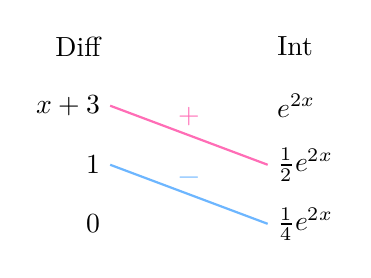
\begin{tikzpicture}[yscale=0.75]
      \draw (-1, 1) node[left]{Diff};
      \draw (1,  1) node[right]{Int};
      \draw (-1, -0) node[left]{$x+3$};
      \draw (1,  -0) node[right]{$e^{2x}$};
      \draw (-1, -1) node[left]{$1$};
      \draw (-1, -2) node[left]{$0$};
      \draw (1,  -1) node[right]{$\frac{1}{2}e^{2x}$};
      \draw (1,  -2) node[right]{$\frac{1}{4}e^{2x}$};
      \draw[thick, M4, -] (-1, -0)--(1, -1); \draw[M4] (0, -0.5) node[above]{$+$};
      \draw[thick, C4, -] (-1, -1)--(1, -2); \draw[C4] (0, -1.5) node[above]{$-$};
    \end{tikzpicture}
  \end{minipage}
  \hspace{5mm}
  \begin{minipage}{0.5\textwidth}
     $\ds\int (x + 3)\,e^{2x}\,\mathrm{d}x = (x + 3)\,\frac{1}{2}e^{2x} - \frac{1}{4}e^{2x}$
  \end{minipage}
\end{sol}

\begin{ex}
  求 $\ds\int (x^2 - 2x)\,e^{kx}\,\mathrm{d}x$。
\end{ex}

\begin{sol} 
  \begin{minipage}{0.35\textwidth}
    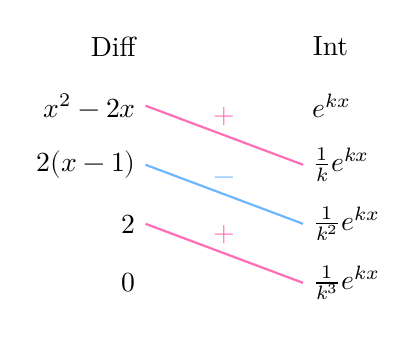
\begin{tikzpicture}[yscale=0.75]
      \draw (-1, 1) node[left]{Diff};
      \draw (1,  1) node[right]{Int};
      \draw (-1, -0) node[left]{$x^2 - 2x$};
      \draw (1,  -0) node[right]{$e^{kx}$};
      \draw (-1, -1) node[left]{$2(x - 1)$};
      \draw (-1, -2) node[left]{$2$};
      \draw (-1, -3) node[left]{$0$};
      \draw (1,  -1) node[right]{$\frac{1}{k}e^{kx}$};
      \draw (1,  -2) node[right]{$\frac{1}{k^2}e^{kx}$};
      \draw (1,  -3) node[right]{$\frac{1}{k^3}e^{kx}$};
      \draw[thick, M4, -] (-1, -0)--(1, -1); \draw[M4] (0, -0.5) node[above]{$+$};
      \draw[thick, C4, -] (-1, -1)--(1, -2); \draw[C4] (0, -1.5) node[above]{$-$};
      \draw[thick, M4, -] (-1, -2)--(1, -3); \draw[M4] (0, -2.5) node[above]{$+$};
    \end{tikzpicture}
  \end{minipage}
  \hspace{5mm}
  \begin{minipage}{0.6\textwidth}
    $\ds\int (x^2 - 2x)\,e^{kx}\,\mathrm{d}x = (x^2 - 2x)\,\frac{1}{k}e^{kx} - 2(x-1)\frac{1}{k^2}e^{kx} + 2\frac{1}{k^3}e^{kx}$
  \end{minipage}
\end{sol}

\begin{ex}
  求 $\ds\int x^4\,\sin 2x\,\mathrm{d}x$。
\end{ex}

\begin{sol} 
  \begin{minipage}{0.25\textwidth}
    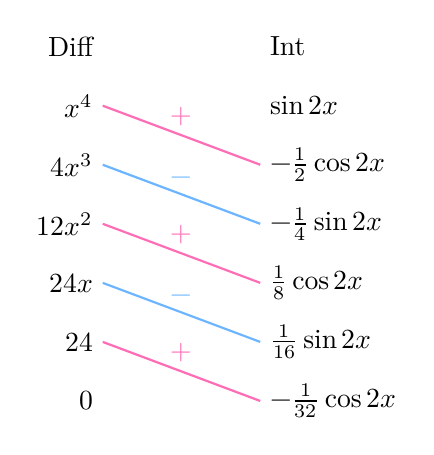
\begin{tikzpicture}[yscale=0.75]
      \draw (-1, 1) node[left]{Diff};
      \draw (1,  1) node[right]{Int};
      \draw (-1, -0) node[left]{$x^4$};
      \draw (1,  -0) node[right]{$\sin 2x$};
      \draw (-1, -1) node[left]{$4x^3$};
      \draw (-1, -2) node[left]{$12x^2$};
      \draw (-1, -3) node[left]{$24x$};
      \draw (-1, -4) node[left]{$24$};
      \draw (-1, -5) node[left]{$0$};
      \draw (1,  -1) node[right]{$-\frac{1}{2}\cos 2x$};
      \draw (1,  -2) node[right]{$-\frac{1}{4}\sin 2x$};
      \draw (1,  -3) node[right]{$\frac{1}{8}\cos 2x$};
      \draw (1,  -4) node[right]{$\frac{1}{16}\sin 2x$};
      \draw (1,  -5) node[right]{$-\frac{1}{32}\cos 2x$};
      \draw[thick, M4, -] (-1, -0)--(1, -1); \draw[M4] (0, -0.5) node[above]{$+$};
      \draw[thick, C4, -] (-1, -1)--(1, -2); \draw[C4] (0, -1.5) node[above]{$-$};
      \draw[thick, M4, -] (-1, -2)--(1, -3); \draw[M4] (0, -2.5) node[above]{$+$};
      \draw[thick, C4, -] (-1, -3)--(1, -4); \draw[C4] (0, -3.5) node[above]{$-$};
      \draw[thick, M4, -] (-1, -4)--(1, -5); \draw[M4] (0, -4.5) node[above]{$+$};
    \end{tikzpicture}
  \end{minipage}
  \hspace{5mm}
  \begin{minipage}{0.7\textwidth}
    $\ds\int x^4\,\sin 2x\,\mathrm{d}x \\= -x^4\,\frac{1}{2}\cos 2x + 4x^3\,\frac{1}{4}\sin 2x + 12x^2\,\frac{1}{8}\cos 2x - 24x\,\frac{1}{16}\sin 2x - 24\,\frac{1}{32}\cos 2x \\= \bigg(-\frac{x^4}{2} + \frac{3x^2}{2} - \frac{3}{4}\bigg)\cos 2x\,+\,\bigg(x^3-\frac{3x}{2}\bigg)\sin 2x$
  \end{minipage}
\end{sol}

\begin{ex}
  求 $\ds\int x^5\,e^{ax}\,\mathrm{d}x$。
\end{ex}

\begin{sol} 
  \begin{minipage}{0.3\textwidth}
    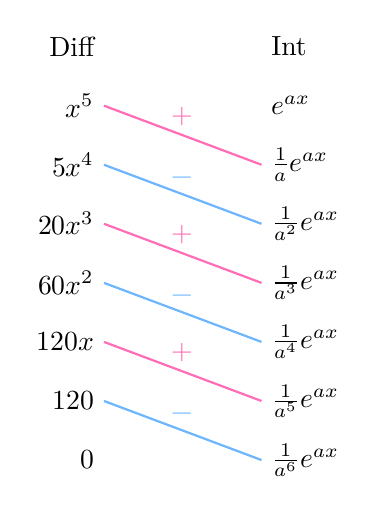
\begin{tikzpicture}[yscale=0.75]
      \draw (-1, 1) node[left]{Diff};
      \draw (1,  1) node[right]{Int};
      \draw (-1, -0) node[left]{$x^5$};
      \draw (1,  -0) node[right]{$e^{ax}$};
      \draw (-1, -1) node[left]{$5x^4$};
      \draw (-1, -2) node[left]{$20x^3$};
      \draw (-1, -3) node[left]{$60x^2$};
      \draw (-1, -4) node[left]{$120x$};
      \draw (-1, -5) node[left]{$120$};
      \draw (-1, -6) node[left]{$0$};
      \draw (1,  -1) node[right]{$\frac{1}{a}e^{ax}$};
      \draw (1,  -2) node[right]{$\frac{1}{a^2}e^{ax}$};
      \draw (1,  -3) node[right]{$\frac{1}{a^3}e^{ax}$};
      \draw (1,  -4) node[right]{$\frac{1}{a^4}e^{ax}$};
      \draw (1,  -5) node[right]{$\frac{1}{a^5}e^{ax}$};
      \draw (1,  -6) node[right]{$\frac{1}{a^6}e^{ax}$};
      \draw[thick, M4, -] (-1, -0)--(1, -1); \draw[M4] (0, -0.5) node[above]{$+$};
      \draw[thick, C4, -] (-1, -1)--(1, -2); \draw[C4] (0, -1.5) node[above]{$-$};
      \draw[thick, M4, -] (-1, -2)--(1, -3); \draw[M4] (0, -2.5) node[above]{$+$};
      \draw[thick, C4, -] (-1, -3)--(1, -4); \draw[C4] (0, -3.5) node[above]{$-$};
      \draw[thick, M4, -] (-1, -4)--(1, -5); \draw[M4] (0, -4.5) node[above]{$+$};
      \draw[thick, C4, -] (-1, -5)--(1, -6); \draw[C4] (0, -5.5) node[above]{$-$};
    \end{tikzpicture}
  \end{minipage}
  \hspace{5mm}
  \begin{minipage}{0.65\textwidth}
    $\ds\int x^5\,e^{ax}\,\mathrm{d}x \\ = x^5\,\frac{1}{a}e^{ax} - 5x^4\,\frac{1}{a^2}e^{ax} + 20x^3\,\frac{1}{a^3}e^{ax} - 60x^2\,\frac{1}{a^4}e^{ax} + 120x\,\frac{1}{a^5}e^{ax} - 120\,\frac{1}{a^6}e^{ax} \\ = \bigg(\frac{x^5}{a}-\frac{5x^4}{a^2} + \frac{20x^3}{a^3} - \frac{60x^2}{a^4} + \frac{120x}{a^5} - \frac{120}{a^6}\bigg)\,e^{ax}$
  \end{minipage}
\end{sol}

\begin{ex}
  求 $\ds\int(\sin^{-1} x)^2\,\mathrm{d}x$。
\end{ex}

\begin{sol} 
  \begin{minipage}{0.35\textwidth}
    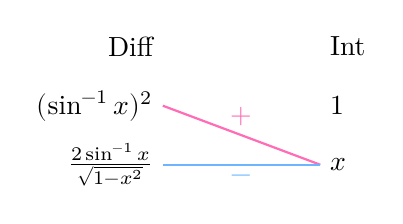
\begin{tikzpicture}[yscale=0.75]
      \draw (-1, 1) node[left]{Diff};
      \draw (1,  1) node[right]{Int};
      \draw (-1, -0) node[left]{$(\sin^{-1} x)^2$};
      \draw (1,  -0) node[right]{$1$};
      \draw (-1, -1) node[left]{$\frac{2\sin^{-1} x}{\sqrt{1-x^2}}$};
      \draw (1,  -1) node[right]{$x$};
      \draw[thick, M4, -] (-1, -0)--(1, -1); \draw[M4] (0, -0.5) node[above]{$+$};
      \draw[thick, C4, -] (-1, -1)--(1, -1); \draw[C4] (0, -1) node[below]{$-$};
    \end{tikzpicture}
    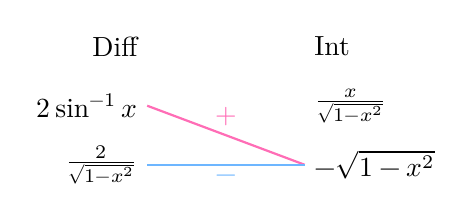
\begin{tikzpicture}[yscale=0.75]
      \draw (-1, 1) node[left]{Diff};
      \draw (1,  1) node[right]{Int};
      \draw (-1, -0) node[left]{$2\sin^{-1} x$};
      \draw (1,  -0) node[right]{$\frac{x}{\sqrt{1-x^2}}$};
      \draw (-1, -1) node[left]{$\frac{2}{\sqrt{1-x^2}}$};
      \draw (1,  -1) node[right]{$-\sqrt{1 - x^2}$};
      \draw[thick, M4, -] (-1, -0)--(1, -1); \draw[M4] (0, -0.5) node[above]{$+$};
      \draw[thick, C4, -] (-1, -1)--(1, -1); \draw[C4] (0, -1) node[below]{$-$};
    \end{tikzpicture}
  \end{minipage}
  \hspace{5mm}
  \begin{minipage}{0.6\textwidth}
    $\ds\int(\sin^{-1} x)^2\,\mathrm{d}x = (\sin^{-1} x)^2\cdot x - \int\frac{2\sin^{-1} x}{\sqrt{1-x^2}}\cdot x\,\mathrm{d}x \\= (\sin^{-1} x)^2\cdot x - \int 2\sin^{-1} x\cdot\frac{x}{\sqrt{1-x^2}}\,\mathrm{d}x \\= (\sin^{-1} x)^2\cdot x - \bigg(-2\sin^{-1} x\cdot\sqrt{1-x^2} + \int \frac{2}{\sqrt{1-x^2}}\cdot\sqrt{1-x^2}\,\mathrm{d}x\bigg)\\ = (\sin^{-1} x)^2\cdot x + 2\sin^{-1} x\cdot\sqrt{1-x^2} - 2x$
  \end{minipage}
\end{sol}

\begin{ex}
  求 $\ds\int e^{ax}\cos bx\,\mathrm{d}x$。
\end{ex}

\begin{sol} 
  \begin{minipage}{0.35\textwidth}
    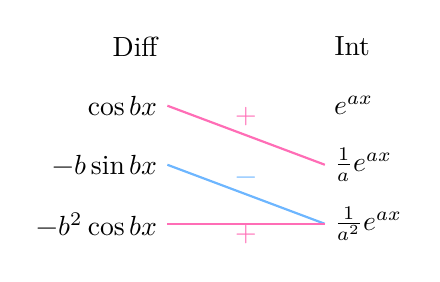
\begin{tikzpicture}[yscale=0.75]
      \draw (-1, 1) node[left]{Diff};
      \draw (1,  1) node[right]{Int};
      \draw (-1, -0) node[left]{$\cos bx$};
      \draw (1,  -0) node[right]{$e^{ax}$};
      \draw (-1, -1) node[left]{$-b\sin bx$};
      \draw (-1, -2) node[left]{$-b^2\cos bx$};
      \draw (1,  -1) node[right]{$\frac{1}{a}e^{ax}$};
      \draw (1,  -2) node[right]{$\frac{1}{a^2}e^{ax}$};
      \draw[thick, M4, -] (-1, -0)--(1, -1); \draw[M4] (0, -0.5) node[above]{$+$};
      \draw[thick, C4, -] (-1, -1)--(1, -2); \draw[C4] (0, -1.5) node[above]{$-$};
      \draw[thick, M4, -] (-1, -2)--(1, -2); \draw[M4] (0, -2.5) node[above]{$+$};
    \end{tikzpicture}
  \end{minipage}
  \hspace{5mm}
  \begin{minipage}{0.6\textwidth}
    $\ds\int e^{ax}\cos bx\,\mathrm{d}x = \frac{1}{a}e^{ax}\cos bx + \frac{b}{a^2}e^{ax}\sin bx - \frac{b^2}{a^2}\int e^{ax}\cos bx\,\mathrm{d}x\\ \ie\int e^{ax}\cos bx\,\mathrm{d}x = \frac{e^{ax}(a\cos bx + b\sin bx)}{a^2 + b^2}$
  \end{minipage}
\end{sol}

\begin{ex}
  求 $\ds\int e^{ax}\sin bx\,\mathrm{d}x$。
\end{ex}

\begin{sol} 
  \begin{minipage}{0.35\textwidth}
    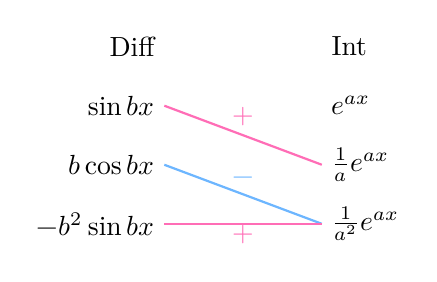
\begin{tikzpicture}[yscale=0.75]
      \draw (-1, 1) node[left]{Diff};
      \draw (1,  1) node[right]{Int};
      \draw (-1, -0) node[left]{$\sin bx$};
      \draw (1,  -0) node[right]{$e^{ax}$};
      \draw (-1, -1) node[left]{$b\cos bx$};
      \draw (-1, -2) node[left]{$-b^2\sin bx$};
      \draw (1,  -1) node[right]{$\frac{1}{a}e^{ax}$};
      \draw (1,  -2) node[right]{$\frac{1}{a^2}e^{ax}$};
      \draw[thick, M4, -] (-1, -0)--(1, -1); \draw[M4] (0, -0.5) node[above]{$+$};
      \draw[thick, C4, -] (-1, -1)--(1, -2); \draw[C4] (0, -1.5) node[above]{$-$};
      \draw[thick, M4, -] (-1, -2)--(1, -2); \draw[M4] (0, -2.5) node[above]{$+$};
    \end{tikzpicture}
  \end{minipage}
  \hspace{5mm}
  \begin{minipage}{0.6\textwidth}
    $\ds\int e^{ax}\sin bx\,\mathrm{d}x = \frac{1}{a}e^{ax}\sin bx - \frac{b}{a^2}e^{ax}\cos bx - \frac{b^2}{a^2}\int e^{ax}\sin bx\,\mathrm{d}x\\ \ie\int e^{ax}\sin bx\,\mathrm{d}x = \frac{e^{ax}(a\sin bx - b\cos bx)}{a^2 + b^2}$
  \end{minipage}
\end{sol}

\begin{exe} 以部份積分法求下列不定積分。注意:可能會因為常數項而跟此處答案不同。
  \begin{enumerate}\setlength\itemsep{0em}
    %\item $\ds\int(x+3)e^{2x}\,\mathrm{d}x {\color{C2}\;= \frac{(x+3)e^{2x}}{2}-\frac{e^{2x}}{4} + c}$
    %\item $\ds\int(x^2 - 2x)e^{kx}\,\mathrm{d}x {\color{C2}\;= \frac{(x^2-2x)e^{kx}}{k} + \frac{2(x-1)e^{kx}}{k^2} + \frac{2e^{kx}}{k^3} + c}$
    \item $\ds\int x(\ln x)^3\,\mathrm{d}x {\color{C2}\;= \frac{x^2}{2}\Big((\ln x)^3 -\frac{3(\ln x)^2}{2} + \frac{3\ln x}{2} - \frac{3}{4} \Big) + c}$
    \item $\ds\int x^2\tan^{-1} x\,\mathrm{d}x {\color{C2}\;= \frac{x^3}{3}\tan^{-1} x - \frac{x^2}{6} + \frac{\ln(1 + x^2)}{6} + c}$
    \item $\ds\int x^5 e^{-x^2}\,\mathrm{d}x {\color{C2}\;= -\frac{1}{2}e^{-x^2}(x^4 + 2x^2 + 2) + c}$
    \item $\ds\int x e^{\sqrt{x}}\,\mathrm{d}x {\color{C2}\;= 2\,e^{\sqrt{x}}\,\big(x\sqrt{x} - 3x + 6\sqrt{x} - 6\big) + c}$
    %\item $\ds\int(\sin^{-1} x)^2\,\mathrm{d}x {\color{C2}\;= x\,(\sin^{-1} x)^2 + 2\sqrt{1 - x^2}\,\sin^{-1} x - 2x + c}$
    \item $\ds\int\sin(\ln x)\,\mathrm{d}x {\color{C2}\;= \frac{x\,(\sin(\ln x) - \cos(\ln x))}{2} + c}$
    \item $\ds\int\frac{\ln x}{\sqrt{1 + x}}\,\mathrm{d}x {\color{C2}\;= \ln x\cdot 2\sqrt{1 + x} - 4\sqrt{1+x} - 2\ln(\sqrt{1 + x}-1) + 2\ln(\sqrt{1+x} + 1) + c}$
  \end{enumerate}
\end{exe}

\begin{sol}
  \begin{enumerate}\setlength\itemsep{0em}
    \item[]
    \item 令 $\ds u = (\ln x)^3$,則 $\ds\text{d}u = 3(\ln x)^2\cdot\frac{1}{x}\,\text{d}x$;$\ds\text{d}v = x\,\text{d}x$,則 $\ds v = \frac{x^2}{2}$。 故 $\ds\int x(\ln x)^3\,\mathrm{d}x = (\ln x)^3\cdot\frac{x^2}{2} - \int\frac{x^2}{2}\cdot 3(\ln x)^2\cdot\frac{1}{x}\,\text{d}x = (\ln x)^3\cdot\frac{x^2}{2} - \frac{3}{2}\int x(\ln x)^2\,\text{d}x$。令 $\ds u = (\ln x)^2$,則 $\ds\text{d}u = 2\,\ln x\cdot\frac{1}{x}\,\text{d}x$;$\ds\text{d}v = x\,\text{d}x$,則 $\ds v = \frac{x^2}{2}$。 故 $\ds\int x(\ln x)^2\,\text{d}x = (\ln x)^2\cdot\frac{x^2}{2} - \int\frac{x^2}{2}\cdot 2\ln x\cdot\frac{1}{x}\,\text{d}x = (\ln x)^2\cdot\frac{x^2}{2} - \int x\ln x\,\text{d}x$。令 $\ds u = \ln x$,則 $\ds\text{d}u = \frac{1}{x}\,\text{d}x$;$\ds\text{d}v = x\,\text{d}x$,則 $\ds v = \frac{x^2}{2}$。故 $\ds\int x\ln x\,\text{d}x = \ln x\cdot\frac{x^2}{2} - \int\frac{x^2}{2}\cdot\frac{1}{x}\,\text{d}x = \ln x\cdot\frac{x^2}{2} - \frac{1}{2}\int x\,\text{d}x = \ln x\cdot\frac{x^2}{2} - \frac{x^2}{4}$。以上,$\ds\int x(\ln x)^3\,\mathrm{d}x = (\ln x)^3\cdot\frac{x^2}{2} - \frac{3}{2}\Big((\ln x)^2\cdot\frac{x^2}{2} - \big(\ln x\cdot\frac{x^2}{2} - \frac{x^2}{4}\big)\Big) = \frac{x^2}{2}\big((\ln x)^3 - \frac{3(\ln x)^2}{2} + \frac{3\ln x}{2} - \frac{3}{4}\big) + c$
    \item 令 $\ds u = \tan^{-1} x$,則 $\ds\text{d}u = \frac{1}{1 + x^2}\,\text{d}x$;$\ds\text{d}v = x^2\,\text{d}x$,則 $\ds v = \frac{x^3}{3}$。 故 $\ds\int x^2\tan^{-1} x\,\mathrm{d}x = \tan^{-1}x\cdot\frac{x^3}{3} - \int\frac{x^3}{3}\cdot\frac{1}{x^2 + 1}\,\text{d}x$。又 $\ds\int\frac{x^3}{3}\cdot\frac{1}{x^2 + 1}\,\text{d}x = \frac{1}{3}\int\frac{(x^3 + x) - x}{x^2 + 1}\,\text{d}x = \frac{1}{3}\int\frac{x(x^2 + 1) - x}{x^2 + 1}\,\text{d}x = \frac{1}{3}\int\big(x - \frac{x}{x^2 + 1}\big)\,\text{d}x$。令 $\ds w = x^2 + 1$,則 $\ds\text{d}w = 2x\,\text{d}x\ie x\,\text{d}x = \frac{1}{2}\,\text{d}w$,故 $\ds\int\frac{x}{x^2 + 1}\,\text{d}x = \int\frac{1}{x^2 + 1}\cdot x\,\text{d}x = \int\frac{1}{w}\cdot\frac{1}{2}\,\text{d}w = \frac{1}{2}\ln w + c = \frac{1}{2}\ln(x^2 + 1) + c$。以上,$\ds\int x^2\tan^{-1} x\,\mathrm{d}x = \tan^{-1}x\cdot\frac{x^3}{3} - \int\frac{x^3}{3}\cdot\frac{1}{x^2 + 1}\,\text{d}x = \tan^{-1}x\cdot\frac{x^3}{3} - \frac{x^2}{6} + \frac{\ln(x^2 + 1)}{6} + c$。
    \item 令 $\ds w = x^2$,則 $\ds\text{d}w = 2x\,\text{d}x\ie x\,\text{d}x = \frac{1}{2}\,\text{d}w$,故 $\ds\int x^5 e^{-x^2}\,\text{d}x = \int e^{-x^2}\cdot(x^2)^2\cdot x\,\text{d}x = \int e^{-w}\cdot w^2\cdot\frac{1}{2}\,\text{d}w = \frac{1}{2}\int w^2\,e^{-w}\,\text{d}w = -\frac{1}{2}\,e^{-w}(w^2 + 2w + 2) = -\frac{1}{2}\,e^{-x^2}(x^4 + 2x^2 + 2) + c$。\\
  \begin{minipage}{0.15\textwidth}
    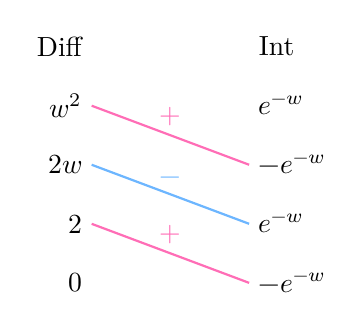
\begin{tikzpicture}[yscale=0.75]
      \draw (-1, 1) node[left]{Diff};
      \draw (1,  1) node[right]{Int};
      \draw (-1, -0) node[left]{$w^2$};
      \draw (1,  -0) node[right]{$e^{-w}$};
      \draw (-1, -1) node[left]{$2w$};
      \draw (-1, -2) node[left]{$2$};
      \draw (-1, -3) node[left]{$0$};
      \draw (1,  -1) node[right]{$-e^{-w}$};
      \draw (1,  -2) node[right]{$e^{-w}$};
      \draw (1,  -3) node[right]{$-e^{-w}$};
      \draw[thick, M4, -] (-1, -0)--(1, -1); \draw[M4] (0, -0.5) node[above]{$+$};
      \draw[thick, C4, -] (-1, -1)--(1, -2); \draw[C4] (0, -1.5) node[above]{$-$};
      \draw[thick, M4, -] (-1, -2)--(1, -3); \draw[M4] (0, -2.5) node[above]{$+$};
    \end{tikzpicture}
  \end{minipage}
  \hspace{5mm}
  \begin{minipage}{0.8\textwidth}
    \begin{align*}
      \int w^2 e^{-w}\,\mathrm{d}w = -w^2\,e^{-w} - 2w\,e^{-w} - 2\,e^{-w} = -e^{-w}(w^2 + 2w + 2)
    \end{align*}
  \end{minipage}
\item 令 $\ds w = \sqrt{x}$,則 $\ds w^2 = x$,$\ds\text{d}x = 2w\,\text{d}w$,故 $\ds\int x e^{\sqrt{x}}\,\mathrm{d}x = \int w^2 e^w\cdot 2w\,\text{d}w = 2\int w^3 e^w\,\text{d}w = 2\,e^w(w^3 - 3w^2 + 6w - 6) = 2\,e^{\sqrt{x}}\,(x\sqrt{x} - 3 x + 6\sqrt{x} - 6) + c$ \\ 
  \begin{minipage}{0.15\textwidth}
    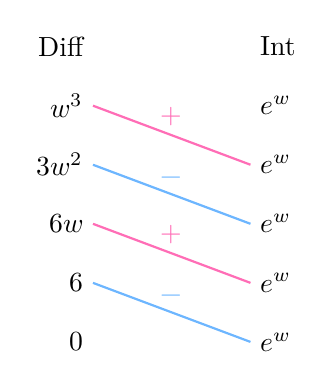
\begin{tikzpicture}[yscale=0.75]
      \draw (-1, 1) node[left]{Diff};
      \draw (1,  1) node[right]{Int};
      \draw (-1, -0) node[left]{$w^3$};
      \draw (1,  -0) node[right]{$e^w$};
      \draw (-1, -1) node[left]{$3w^2$};
      \draw (-1, -2) node[left]{$6w$};
      \draw (-1, -3) node[left]{$6$};
      \draw (-1, -4) node[left]{$0$};
      \draw (1,  -1) node[right]{$e^w$};
      \draw (1,  -2) node[right]{$e^w$};
      \draw (1,  -3) node[right]{$e^w$};
      \draw (1,  -4) node[right]{$e^w$};
      \draw[thick, M4, -] (-1, -0)--(1, -1); \draw[M4] (0, -0.5) node[above]{$+$};
      \draw[thick, C4, -] (-1, -1)--(1, -2); \draw[C4] (0, -1.5) node[above]{$-$};
      \draw[thick, M4, -] (-1, -2)--(1, -3); \draw[M4] (0, -2.5) node[above]{$+$};
      \draw[thick, C4, -] (-1, -3)--(1, -4); \draw[C4] (0, -3.5) node[above]{$-$};
    \end{tikzpicture}
  \end{minipage}
  \hspace{5mm}
  \begin{minipage}{0.8\textwidth}
    \begin{align*}
      \int w^3\,e^w\,\mathrm{d}w = w^3\,e^w - 3w^2\,e^w + 6w\,e^w - 6\,e^w = e^w(w^3 - 3w^2 + 6w - 6)
    \end{align*}
  \end{minipage}
    %\item 令 $\ds u = (\sin^{-1} x)^2$,則 $\ds\text{d}u = 2\sin^{-1}x\frac{1}{\sqrt{1 - x^2}}\,\text{d}x$;$\ds\text{d}v = \text{d}x$,則 $\ds v = x$。 故 $\ds\int(\sin^{-1} x)^2\,\text{d}x = (\sin^{-1} x)^2\cdot x - \int x\cdot 2\sin^{-1}x\frac{1}{\sqrt{1 - x^2}}\,\text{d}x = (\sin^{-1} x)^2\cdot x + 2\int\sin^{-1}x\cdot\frac{-x}{\sqrt{1 - x^2}}\,\text{d}x$。令 $\ds u = \sin^{-1} x$,則 $\ds\text{d}u = \frac{1}{\sqrt{1 - x^2}}\,\text{d}x$;$\ds\text{d}v = \frac{-x}{\sqrt{1 - x^2}}\,\text{d}x$,則 $\ds v = \sqrt{1 - x^2}$。 故 $\ds\int\sin^{-1}x\cdot\frac{-x}{\sqrt{1 - x^2}}\,\text{d}x = \sin^{-1}x\cdot\sqrt{1 - x^2} - \int\sqrt{1 - x^2}\cdot\frac{1}{\sqrt{1 - x^2}}\,\text{d}x = \sin^{-1}x\cdot\sqrt{1 - x^2} - \int 1\,\text{d}x = \sin^{-1}x\cdot\sqrt{1 - x^2} - x$。以上,$\ds\int(\sin^{-1} x)^2\,\text{d}x = (\sin^{-1} x)^2\cdot x + 2\,(\sin^{-1}x\cdot\sqrt{1 - x^2} - x) = x\,(\sin^{-1} x)^2 + 2\sqrt{1 - x^2}\,\sin^{-1}x - 2x + c$
    \item 令 $\ds w = \ln x$,則 $\ds e^w = x$,$\ds\text{d}x = e^w\,\text{d}w$,故 $\ds\int\sin(\ln x)\,\text{d}x = \int\sin w\cdot e^w\,\text{d}w = \int e^w\,\sin w\,\text{d}w = \frac{e^w(\sin w - \cos w)}{2} = \frac{x\,(\sin(\ln x) - \cos(\ln x))}{2} + c$ \\
      \begin{minipage}{0.15\textwidth}
        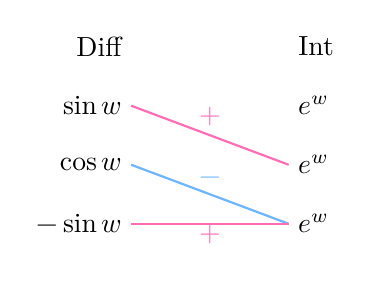
\begin{tikzpicture}[yscale=0.75]
          \draw (-1, 1) node[left]{Diff};
          \draw (1,  1) node[right]{Int};
          \draw (-1, -0) node[left]{$\sin w$};
          \draw (1,  -0) node[right]{$e^w$};
          \draw (-1, -1) node[left]{$\cos w$};
          \draw (-1, -2) node[left]{$-\sin w$};
          \draw (1,  -1) node[right]{$e^w$};
          \draw (1,  -2) node[right]{$e^w$};
          \draw[thick, M4, -] (-1, -0)--(1, -1); \draw[M4] (0, -0.5) node[above]{$+$};
          \draw[thick, C4, -] (-1, -1)--(1, -2); \draw[C4] (0, -1.5) node[above]{$-$};
          \draw[thick, M4, -] (-1, -2)--(1, -2); \draw[M4] (0, -2.5) node[above]{$+$};
        \end{tikzpicture}
      \end{minipage}
      \hspace{5mm}
      \begin{minipage}{0.8\textwidth}
        \begin{align*}
          &\int e^w\sin w\,\mathrm{d}w = e^{w}\sin w - e^w\cos w - \int e^w\sin w\,\mathrm{d}w\\ 
          &\ie\int e^w\sin w\,\mathrm{d}w = \frac{e^w(\sin w - \cos w)}{2}
        \end{align*}
      \end{minipage}
    \item 令 $\ds u = \ln x$,則 $\ds\text{d}u = \frac{1}{x}\,\text{d}x$;$\ds\text{d}v = \frac{1}{\sqrt{1 + x}}\,\text{d}x$,則 $\ds v = 2\sqrt{1 + x}$。故 $\ds\int\frac{\ln x}{\sqrt{1 + x}}\,\text{d}x = \ln x\cdot 2\sqrt{1 + x} - 2 \int\frac{\sqrt{1 + x}}{x}\,\text{d}x$。令 $\ds w = \sqrt{1 + x}$,則 $\ds w^2 = 1 + x \ie x= w^2 - 1$,$\ds 2w\,\text{d}w = \text{d}x$,故 $\ds\int\frac{\sqrt{1 + x}}{x}\,\text{d}x = \int\frac{w}{w^2 - 1}\cdot 2w\,\text{d}w = 2\int\frac{w^2}{w^2 - 1}\,\text{d}w = 2\int\frac{(w^2 - 1) + 1}{w^2 - 1}\,\text{d}w = 2 w + 2\int\frac{1}{w^2 - 1}\,\text{d}w = 2\sqrt{1 + x} + 2\int\frac{1}{w^2 -1}\,\text{d}w$。由部份分式 $\ds\frac{1}{w^2 - 1} = \frac{1}{2}\,\Big(\frac{1}{w - 1} - \frac{1}{w + 1}\Big)$,$\ds\int\frac{1}{w^2 - 1}\,\text{d}w = \frac{1}{2}\int\Big(\frac{1}{w - 1} - \frac{1}{w + 1}\Big)\,\text{d}w =\frac{1}{2}\,\big(\ln(w - 1) - \ln(w + 1)\big) = \frac{1}{2}\,\big(\ln(\sqrt{1 + x} - 1) - \ln(\sqrt{1 + x} + 1)\big)$。以上,$\ds\int\frac{\ln x}{\sqrt{1 + x}}\,\mathrm{d}x = \ln x\cdot 2\sqrt{1 + x} - 2\,\big(2\sqrt{1+x} + 2\,\big(\frac{1}{2}\,\big(\ln(\sqrt{1 + x}-1) - \ln(\sqrt{1+x} + 1)\big)\big)\big) = \ln x\cdot 2\sqrt{1 + x} - 4\sqrt{1+x} - 2\ln(\sqrt{1 + x}-1) + 2\ln(\sqrt{1+x} + 1) + c$。
  \end{enumerate}
\end{sol}

\myline

\section*{4.2 定積分}

\begin{figure}[!htbp]
  \centering
  \includegraphics[scale=1,page=1]{fig/lu.pdf}
  \includegraphics[scale=1,page=2]{fig/lu.pdf}
\end{figure}

\begin{dfn}
  令 $f$ 在 $[a,b]$ 連續。
  \begin{itemize}\setlength\itemsep{0em}
    \item $\ds\mathbb{P}: a = x_0 < x_1 < x_2 < \cdots < x_n = b$ 為 $[a, b]$ 的分割。
    \item $\ds\Delta x_k=x_k - x_{k-1}$,$\ds\|\mathbb{P}\| = \max\{\,|\Delta x_k|\;|\;1\leqslant k\leqslant n\}$,$\ds x_{k-1}\leqslant \xi_k \leqslant x_k$,$k=1,2,\ldots,n$
    \item $\ds u_k = \sup\left\{\,f(x)\;|\;x_{k-1}\leqslant x\leqslant x_k\right\}$,$l_k = \inf\left\{\,f(x)\;|\;x_{k-1}\leqslant x\leqslant x_k\right\}$,$k=1,2,\ldots,n$
    \item $\ds R(f,\mathbb{P}) = \sum_{k=1}^n f(\xi_k)\,\Delta x_k$,$\ds U(f,\mathbb{P}) = \sum_{k=1}^n u_k\,\Delta x_k$,$\ds L(f,\mathbb{P}) = \sum_{k=1}^n l_k\,\Delta x_k$;\\顯然 $\ds L(f,\mathbb{P})\leqslant R(f,\mathbb{P})\leqslant U(f, \mathbb{P})$。
    \item $\ds\int_a^b f(x)\,\mathrm{d}x\equiv\lim_{\substack{n\to\infty \\ \|\mathbb{P}\|\to 0}} R(f,\mathbb{P})$;若此極限存在,稱 $f$ 在 $[a, b]$ 可積(分)。
  \end{itemize}
\end{dfn}

\begin{prp}[定積分基本性質]
  令 $f$、$g$ 在包含 $a$、$b$、$c$ 之區間為可積,$\alpha$、$\beta\in\mathbb{R}$。則
  \begin{enumerate}\setlength\itemsep{0em}
    \item $\ds\int_a^a f(x)\,\mathrm{d}x = 0$
    \item $\ds\int_a^b f(x)\,\mathrm{d}x = -\int_b^a f(x)\,\mathrm{d}x$
    \item $\ds\int_a^b \big(\alpha\,f(x) + \beta\,g(x)\big)\,\mathrm{d}x = \alpha\int_a^b f(x)\,\mathrm{d}x + \beta\int_a^b g(x)\,\mathrm{d}x$
    \item $\ds\int_a^b f(x)\,\mathrm{d}x + \int_b^c f(x)\,\mathrm{d}x = \int_a^c f(x)\,\mathrm{d}x$
    \item $\ds\int_a^b f(x)\,\mathrm{d}x\leqslant\int_a^b g(x)\,\mathrm{d}x$,若 $f(x)\leqslant g(x)\;\forall\,x\in[a, b],\;a\leqslant b$
    \item $\ds\left|\,\int_a^b f(x)\,\mathrm{d}x\,\right|\leqslant \int_a^b \left|\,f(x)\,\right|\,\mathrm{d}x, \quad a\leqslant b$ 
    \item $\ds\int_{-a}^a f(x)\,\mathrm{d}x = 0$,若 $f(x)$ 為奇函數
    \item $\ds\int_{-a}^a f(x)\,\mathrm{d}x = 2\int_0^a f(x)\,\mathrm{d}x$,若 $f(x)$ 為偶函數
  \end{enumerate}
\end{prp}

\begin{ex}
  \begin{enumerate}\setlength\itemsep{0em}
    \item[]
    \item $\ds\int_{-\sqrt{2}}^{\sqrt{2}} \sqrt{2 - x^2}\,\mathrm{d}x = \pi$(半徑 $\sqrt{2}$ 之半圓面積)
    \item $\ds\int_{-1}^2 \sgn(x)\,\mathrm{d}x = 2\cdot 1 - 1\cdot 1 = 1$
    \item $\ds\int_{-\pi}^{\pi} \sin(x^7-5x^3)\,\mathrm{d}x = 0$($\sin(x^7-5x^3)$ 為奇函數)
    \item $\ds\int_{-6}^{6} e^{-x^4}\sin(\sin x)\,\mathrm{d}x = 0$($e^{-x^4}\sin(\sin x)$ 為奇函數)
    \item $\ds\int_{-4}^{4} \big(e^{x} - e^{-x}\big)\,\mathrm{d}x = 0$($e^{x} - e^{-x}$ 為奇函數)
    \item $\ds\int_{-100}^{100} \big(e^{9x^5-2x^7} - e^{-9x^5 + 2x^7}\big)\,\mathrm{d}x = 0$($e^{9x^5-2x^7} - e^{-9x^5 + 2x^7}$ 為奇函數) 
    \item $\ds\int_{-a}^a |x|\,\mathrm{d}x = 2\int_0^a |x|\,\mathrm{d}x = a^2$($|x|$ 為奇函數;兩 $a\times a$ 直角三角形面積)
    \item 定義 $\ds\int_1^x\frac{1}{\tau}\,\mathrm{d}\tau\equiv\ln x$,則 $\ds\int_{\frac{1}{4}}^3\frac{1}{x}\,\mathrm{d}x = \int_{\frac{1}{4}}^1 \frac{1}{x}\,\mathrm{d}x + \int_1^3 \frac{1}{x}\,\mathrm{d}x = -\int_1^{\frac{1}{4}}\frac{1}{x}\,\mathrm{d}x + \int_1^3\frac{1}{x}\,\mathrm{d}x = \ln 12$
    \item $\ds\int_0^2 \sqrt{4 - x^2}\cdot\sgn(x - 1)\,\mathrm{d}x = \pi - \sqrt{3}$ 
  \end{enumerate}
\end{ex}

\begin{fact}
  $\ds\sum_{k = 1}^m k^2 = \frac{m(m + 1)(2m + 1)}{6}$。
\end{fact}

\begin{ex}
  求 $\ds\int_0^1 x^2\,\text{d}x$。
\end{ex}

\begin{sol}
  建立 $\ds [0,\,1]$ 分割 $\ds\mathbb{P}: \Big\{0, \frac{1}{n}, \frac{2}{n}, \ldots, \frac{n}{n}\Big\}$,則 $\ds\Delta x_k = \frac{1}{n}\;\forall\,k=1,2,\ldots,n$ 且 $\ds\|P\|\to 0$ 當 $n\to\infty$。$f(x) = x^2$ 且 $f$ 在 $[0,\,1]$ 嚴格遞增,$\ds U(f,\mathbb{P}) = \sum_{k=1}^n u_k\,\Delta x_k = \sum_{k=1}^n\frac{k^2}{n^2}\cdot\frac{1}{n} = \frac{1}{n^3}\sum_{k = 1}^n k^2$,$\ds L(f,\mathbb{P}) = \sum_{k=1}^n l_k\,\Delta x_k = \sum_{k=1}^n\frac{(k - 1)^2}{n^2}\cdot\frac{1}{n} = \frac{1}{n^3}\sum_{k = 1}^{n-1}k^2$,$\ds L(f,\mathbb{P})\leqslant R(f,\mathbb{P})\leqslant U(f, \mathbb{P})$。由 $\ds\sum_{k = 1}^m k^2 = \frac{m(m + 1)(2m + 1)}{6}$,$\ds\lim_{n\to\infty} U(f,\mathbb{P}) = \lim_{n\to\infty}\frac{1}{n^3}\sum_{k = 1}^n k^2 = \lim_{n\to\infty}\frac{n(n + 1)(2 n + 1)}{6n^3} = \frac{1}{3}$,$\ds\lim_{n\to\infty} L(f,\mathbb{P}) = \lim_{n\to\infty}\frac{1}{n^3}\sum_{k = 1}^{n - 1} k^2 = \lim_{n\to\infty}\frac{(n - 1)n(2 n - 1)}{6n^3} = \frac{1}{3}$,故由夾擊定理 $\ds\lim_{n\to\infty} R(f,\mathbb{P}) = \frac{1}{3}$。
\end{sol}

\begin{fact}
  若 $r\in\mathbb{R}$,$\ds\sum_{k = 0}^n r^k = \frac{r^{n+1} - 1}{r - 1}$。
\end{fact}

\begin{ex}
  求 $\ds\int_0^1 e^x\,\text{d}x$。
\end{ex}

\begin{sol}
  建立 $\ds [0,\,1]$ 分割 $\ds\mathbb{P}: \Big\{0, \frac{1}{n}, \frac{2}{n}, \ldots, \frac{n}{n}\Big\}$,則 $\ds\Delta x_k = \frac{1}{n}\;\forall\,k=1,2,\ldots,n$ 且 $\ds\|P\|\to 0$ 當 $n\to\infty$。$f(x) = e^x$ 且 $f$ 在 $[0,\,1]$ 嚴格遞增,$\ds U(f,\mathbb{P}) = \sum_{k=1}^n u_k\,\Delta x_k = \sum_{k=1}^n e^{\frac{k}{n}}\cdot\frac{1}{n} = \frac{1}{n}\frac{e^{\frac{1}{n}}\big(e^{\frac{n}{n}} - 1\big)}{e^{\frac{1}{n}} - 1} = \frac{e - 1}{n}\frac{e^{\frac{1}{n}}}{e^{\frac{1}{n}} - 1}$,$\ds L(f,\mathbb{P}) = \sum_{k=1}^n l_k\,\Delta x_k = \sum_{k=1}^n e^{\frac{k - 1}{n}}\cdot\frac{1}{n} = \frac{1}{n}\frac{e^0\big(e^{\frac{n}{n}} - 1\big)}{e^{\frac{1}{n}} - 1} = \frac{e - 1}{n}\frac{1}{e^{\frac{1}{n}} - 1}$,$\ds L(f,\mathbb{P})\leqslant R(f,\mathbb{P})\leqslant U(f, \mathbb{P})$。$\ds\lim_{n\to\infty} U(f,\mathbb{P}) = \lim_{n\to\infty}\frac{e - 1}{n}\frac{e^{\frac{1}{n}}}{e^{\frac{1}{n}} - 1} = (e - 1)\lim_{x\to 0+}\frac{x e^x}{e^x - 1} = (e - 1)\lim_{x\to 0+}\frac{e^x + x e^x}{e^x} = e - 1$,$\ds\lim_{n\to\infty} L(f,\mathbb{P}) = \lim_{n\to\infty}\frac{e - 1}{n}\frac{1}{e^{\frac{1}{n}} - 1} = (e - 1)\lim_{x\to 0+}\frac{x}{e^x - 1} = (e - 1)\lim_{x\to 0+}\frac{1}{e^x} = e - 1$,故由夾擊定理 $\ds\lim_{n\to\infty} R(f,\mathbb{P}) = e - 1$。
\end{sol}

\begin{thm}[微積分基本定理(Fundamental Theorem of Calculus,FTC)]
  \begin{enumerate}\setlength\itemsep{0em}
    \item[]
    \item 若 $f$ 在 $[a, b]$ 連續,令 $\ds F(x) = \int_a^x f(\tau)\,\mathrm{d}\tau$ 且 $a\leqslant x\leqslant b$,則 $\ds F'(x) = f(x)\;\forall\,x\in[a, b]$。
    \item 若 $\ds G'(x) = f(x)\;\forall\,x\in[a, b]$,則 $\ds\int_a^b f(x)\,\mathrm{d}x = G(b) - G(a) \equiv G(x)\,\Big|_a^b$。
  \end{enumerate}
\end{thm}
\begin{rmk}
  由 FTC,$\ds\int_a^b f(x)\,\mathrm{d}x$ 可由 $f$ 的反導函數(不定積分)得出,不需繁複極限計算!
\end{rmk}

\begin{prf}
  \begin{enumerate}\setlength\itemsep{0em}
    \item[]
    \item WLOG 令 $h > 0$。則 $\ds\Bigg|\,\frac{F(x + h) - F(x)}{h} - f(x)\,\Bigg| = \Bigg|\,\frac{1}{h}\int_x^{x + h}(f(\tau) - f(x))\,\mathrm{d}\tau\,\Bigg| \leqslant\frac{1}{h}\int_x^{x + h}\big|\,f(\tau) - f(x)\big|\,\mathrm{d}\tau \leqslant\max_{x\leqslant\tau\leqslant x+h}\big|\,f(\tau) - f(x)\big|\to 0$,當 $h\to 0$ 且 $f$ 為連續。
    \item $\ds(G(x) - F(x))' = f(x) - f(x) = 0\;\forall\,x\in[a, b]$,故 $\ds G(x) - F(x)$ 在 $[a, b]$ 為常數 $\ds\ie G(a) - F(a) = G(b) - F(b) \ie G(b) - G(a) = F(b) - F(a) = \int_a^b f(x)\,\mathrm{d}x$。
  \end{enumerate}
\end{prf}

\begin{ex}[由 FTC 求定積分]
  \begin{enumerate}\setlength\itemsep{0em}
    \item[]
    \item $\ds x^2$ 之反導函數為 $\ds\frac{x^3}{3}$,故 $\ds\int_0^1 x^2\,\text{d}x = \frac{1^3}{3} - \frac{0^3}{3} = \frac{1}{3}$。
    \item $\ds e^x$ 之反導函數為 $\ds e^x$,故 $\ds\int_0^1 e^x\,\text{d}x = e^1 - e^0 = e - 1$。
  \end{enumerate}
\end{ex}

\begin{fact}
  $\ds\sum_{k = 1}^n \cos kx = \frac{1}{2}\bigg(\frac{\sin\big(n+\frac{1}{2}\big)x}{\sin\frac{x}{2}}-1\bigg)$
\end{fact}

\begin{prf}
  考慮 $\ds\sum_{k = 1}^{n} e^{ikx} = \frac{e^{ix}(1 - e^{inx})}{1 - e^{ix}}$,則 $\ds\sum_{k = 1}^{n} \cos kx = \Re\Big\{\sum_{k = 1}^n e^{ikx}\Big\} = \Re\Big\{\frac{e^{ix}(1 - e^{inx})}{1 - e^{ix}}\Big\} = \Re\bigg\{\frac{e^{ix}\,e^{\frac{inx}{2}}\big(e^{-\frac{inx}{2}} - e^{\frac{inx}{2}}\big)}{e^{\frac{ix}{2}}\big(e^{-\frac{ix}{2}} - e^{\frac{ix}{2}}\big)}\bigg\} = \frac{\cos\frac{(n+1)x}{2}\,\sin\frac{nx}{2}}{\sin\frac{x}{2}} = \frac{\sin\big(\frac{nx}{2} + \frac{(n + 1)x}{2}\big) + \sin\big(\frac{nx}{2} + \frac{(n + 1)x}{2}\big)}{2\,\sin\frac{x}{2}} = \frac{\sin\big(n+\frac{1}{2}\big)x - \sin\frac{x}{2}}{2\,\sin\frac{x}{2}} = \frac{1}{2}\bigg(\frac{\sin\big(n+\frac{1}{2}\big)x}{\sin\frac{x}{2}}-1\bigg)$。 
\end{prf}

\begin{ex}
  求 $\ds\int_0^{\frac{\pi}{2}}\cos x\,\mathrm{d}x$。
\end{ex}

\begin{sol}
  \begin{itemize}\setlength\itemsep{0em}
    \item[]
    \item(極限定義)建立 $\ds \big[0,\,\frac{\pi}{2}\big]$ 分割 $\ds\mathbb{P}: \big\{0, \frac{\pi}{2n}, \frac{2\pi}{2n}, \ldots, \frac{n\pi}{2n}\big\}$,則 $\ds\Delta x_k = \frac{\pi}{2n}\;\forall\,k=1,2,\ldots,n$ 且 $\ds\|P\|\to 0$ 當 $n\to\infty$,則積分為 $\ds\lim_{n\to\infty} R(f,\mathbb{P}) = \sum_{k=1}^n f(\xi_k)\,\Delta x_k = \lim_{n\to\infty}\sum_{k=1}^n\cos\frac{k\pi}{2n}\cdot\frac{\pi}{2n}  = \lim_{n\to\infty}\sum_{k=1}^n\cos\Big(k\,\big(\frac{\pi}{2n}\big)\Big)\cdot\frac{\pi}{2n} = \\ \lim_{n\to\infty}\frac{1}{2}\bigg(\frac{\sin\big(\big(n+\frac{1}{2}\big)\cdot\frac{\pi}{2n}\big)}{\sin\big(\frac{1}{2}\cdot\frac{\pi}{2n}\big)}-1\bigg)\cdot\frac{\pi}{2n} = \lim_{n\to\infty}\frac{\sin\big(\big(n+\frac{1}{2}\big)\frac{\pi}{2n}\big)\frac{1}{2}\cdot\frac{\pi}{2n}}{\sin\big(\frac{1}{2}\cdot\frac{\pi}{2n}\big)} = \lim_{n\to\infty}\sin\Big(\frac{1}{2} + \frac{1}{4n}\Big)\pi\cdot\lim_{n\to\infty}\frac{\frac{1}{2}\cdot\frac{\pi}{2n}}{\sin\big(\frac{1}{2}\cdot\frac{\pi}{2n}\big)} = \sin\frac{\pi}{2}\cdot 1 = 1$.
    \item(FTC)$\cos x$ 之反導函數為 $\sin x$,故 $\ds\int_0^{\frac{\pi}{2}}\cos x\,\mathrm{d}x = \sin\frac{\pi}{2} - \sin 0 = 1$。
  \end{itemize}
\end{sol}

\begin{prp}
  令 $\ds F(x) = \int_{v(x)}^{u(x)} f(\tau)\,\mathrm{d}\tau$,則 $\ds F'(x) = f(u(x))\cdot u'(x) - f(v(x))\cdot v'(x)$。
\end{prp}

\begin{prf}
  令 $a\in\mathbb{R}$,$\ds F(x) = \int_{v(x)}^{u(x)} f(\tau)\,\mathrm{d}\tau = \int_{a}^{u(x)} f(\tau)\,\mathrm{d}\tau - \int_{a}^{v(x)} f(\tau)\,\mathrm{d}\tau$。令 $\ds G(x)\equiv\int_a^x f(\tau)\,\mathrm{d}\tau$,則 $\ds G'(x) = f(x)$,$\ds F(x) = \int_{a}^{u(x)} f(\tau)\,\mathrm{d}\tau - \int_{a}^{v(x)} f(\tau)\,\mathrm{d}\tau = G(u(x)) - G(v(x))$;故 $\ds F'(x) = (G(u(x)) - G(v(x)))' = G'(u(x))\cdot u'(x) - G'(v(x))\cdot v'(x) = f(u(x))\cdot u'(x) - f(v(x))\cdot v'(x)$。  
\end{prf}

\begin{ex} 
  \begin{enumerate}\setlength\itemsep{0em}
    \item[]
    \item $\ds F(x) = \int_1^x\frac{1}{1 + \tau^4}\,\mathrm{d}\tau \ie F'(x) = \frac{1}{1 + x^4}$ 
    \item $\ds F(x) = \int_2^{\sqrt{x}}\sin\tau\,\mathrm{d}\tau \ie F'(x) = \sin\sqrt{x}\cdot\frac{1}{2\sqrt{x}}$
    \item $\ds F(x) = \int_{x}^{2x}\tau^3\,\mathrm{d}\tau \ie F'(x) = (2x)^3\cdot 2 - x^3\cdot 1 = 15x^3$
  \end{enumerate}
\end{ex}

\subsection*{定積分變數變換}

\begin{fact} 
  \begin{itemize}\setlength\itemsep{0em}
    \item[]
    \item 先求得反導函數後再代入:$\ds\int_a^b f'(g(x))\,g'(x)\,\text{d}x = f(g(x))\,\Big|_{x = a}^{x = b} = f(g(b)) - f(g(a))$
    \item 變數變換並改變積分範圍:$\ds\int_a^b f'(g(x))\,g'(x)\,\text{d}x = \int_a^b f'(g(x))\,\text{d}g(x) =\int_{g(a)}^{g(b)} f'(u)\,\text{d}u = f(u)\,\Big|_{u = g(a)}^{u = g(b)} = f(g(b)) - f(g(a))$
  \end{itemize}
\end{fact}

\begin{ex}
  求 $\ds\int_0^1 x^3(1 + x^4)^3\,\text{d}x$。
\end{ex}

\begin{sol}
  \begin{itemize}\setlength\itemsep{0em}
    \item[]
    \item 先求得反導函數後再代入:令 $\ds u = 1 + x^4$,則 $\ds\text{d}u = 4 x^3\,\text{d}x\ie x^3\,\text{d}x = \frac{\text{d}u}{4}$,故 $\ds\int x^3(1 + x^4)^3\,\text{d}x = \int (1 + x^4)^3\,x^3\,\text{d}x = \int u^3\,\frac{\text{d}u}{4} = \frac{u^4}{16} + c = \frac{(1 + x^4)^4}{16} + c$。故 $\ds\int_0^1 x^3(1 + x^4)^3\,\text{d}x = \frac{(1 + x^4)^4}{16}\,\Big|_{x = 0}^{x = 1} = \frac{(1 + 1^4)^4 - (1 + 0^4)^4}{16} = \frac{15}{16}$。
    \item 變數變換並改變積分範圍:令 $\ds u = 1 + x^4$,則 $\ds\text{d}u = 4 x^3\,\text{d}x\ie x^3\,\text{d}x = \frac{\text{d}u}{4}$。積分範圍 $x$ 由 $0$ 至 $1$,則變數變換後 $u$ 由 $\ds 1 + 0^4 = 1$ 至 $\ds1 + 1^4 = 2$,故 $\ds\int_0^1 x^3(1 + x^4)^3\,\text{d}x = \int_0^1 (1 + x^4)^3\,x^3\,\text{d}x = \int_1^2 u^3\,\frac{\text{d}u}{4} = \frac{1}{4}\int_1^2 u^3\,\text{d}u = \frac{1}{16} u^4\,\Big|_{u = 1}^{u = 2} = \frac{2^4 - 1^4}{16} = \frac{15}{16}$。
  \end{itemize}
\end{sol}

\begin{ex}
  求 $\ds\int_0^{\sqrt{3}}\frac{4x}{\sqrt{1 + x^2}}\,\text{d}x$。
\end{ex}

\begin{sol}
  \begin{itemize}\setlength\itemsep{0em}
    \item[]
    \item 先求得反導函數後再代入:令 $\ds u = 1 + x^2$,則 $\ds\text{d}u = 2 x\,\text{d}x\ie 4x\,\text{d}x = 2\,\text{d}u$,故 $\ds\int\frac{4x}{\sqrt{1 + x^2}}\,\text{d}x = \int\frac{2}{\sqrt{u}}\,\text{d}u = 4\sqrt{u} + c = 4\sqrt{1 + x^2} + c$。故 $\ds\int_0^{\sqrt{3}}\frac{4x}{\sqrt{1 + x^2}}\,\text{d}x = 4\sqrt{1 + x^2}\,\Big|_{x = 0}^{x = \sqrt{3}} = 4\sqrt{1 + 3} - 4\sqrt{1} = 4$。
    \item 變數變換並改變積分範圍:令 $\ds u = 1 + x^2$,則 $\ds\text{d}u = 2 x\,\text{d}x\ie 4x\,\text{d}x = 2\,\text{d}u$。積分範圍 $x$ 由 $0$ 至 $\sqrt{3}$,則變數變換後 $u$ 由 $\ds1 + 0^2 = 1$ 至 $\ds1 + (\sqrt{3})^2 = 4$,故 $\ds\int_0^{\sqrt{3}}\frac{4x}{\sqrt{1 + x^2}}\,\text{d}x = \int_1^4 \frac{2}{\sqrt{u}}\,\text{d}u = 4\sqrt{u}\,\Big|_{u = 1}^{u = 4} = 4\,(\sqrt{4} - \sqrt{1}) = 4$。
  \end{itemize}
\end{sol}

\begin{ex}
  求 $\ds\int_0^{\pi}3\cos^2 x\sin x\,\text{d}x$。
\end{ex}

\begin{sol}
  \begin{itemize}\setlength\itemsep{0em}
    \item[]
    \item 先求得反導函數後再代入:令 $\ds u = \cos x$,則 $\ds\text{d}u = -\sin x\,\text{d}x\ie \sin x\,\text{d}x = -\text{d}u$,故 $\ds\int3\cos^2 x\sin x\,\text{d}x = -3\int u^2\,\text{d}u = -u^3 + c = -\cos^3 x + c$。故 $\ds\int_0^{\pi}3\cos^2 x\sin x\,\text{d}x = -\cos^3 x\,\Big|_{x = 0}^{x = \pi} = -(\cos^3\pi - \cos^3 0) = -((-1)^3 - 1^3) = 2$。
    \item 變數變換並改變積分範圍:令 $\ds u = \cos x$,則 $\ds\text{d}u = -\sin x\,\text{d}x\ie \sin x\,\text{d}x = -\text{d}u$。積分範圍 $x$ 由 $0$ 至 $\pi$,則變數變換後 $u$ 由 $\ds\cos 0 = 1$ 至 $\ds\cos\pi= -1$,故 $\ds\int_0^{\pi}3\cos^2 x\sin x\,\text{d}x = -\int_{1}^{-1}3u^2\,\text{d}u = -u^3\,\Big|_{u = 1}^{u = -1} = -((-1)^3 - 1^3) = 2$。
  \end{itemize}
\end{sol}
\section*{4.3 瑕積分}

\begin{dfn}[瑕積分]
  \begin{itemize}\setlength\itemsep{0em}
    \item[]
    \item 若 (i) $f$ 在 $I$ 有無限函數值或 (ii) $I$ 為無限區間,$\ds\int_I f(x)\,\mathrm{d}x$ 稱為瑕積分(improper integral)。
    \item $\ds\int_{-\infty}^{\infty} f(x)\,\mathrm{d}x = \lim_{\substack{a\to-\infty \\ b\to\infty}}\int_a^b f(x)\,\mathrm{d}x$。
  \end{itemize}
\end{dfn}

\begin{ex}
  求 $\ds\int_{-\infty}^{\infty} \frac{1}{1 + x^2}\,\mathrm{d}x$。
\end{ex}

\begin{sol}
  $\ds\int_{-\infty}^{\infty} \frac{1}{1 + x^2}\,\mathrm{d}x = 2\int_0^\infty\frac{1}{1 + x^2}\,\mathrm{d}x = 2\lim_{b\to\infty}\int_0^b\frac{1}{1 + x^2}\,\mathrm{d}x = 2\lim_{b\to\infty}\tan^{-1} b = 2\cdot\frac{\pi}{2} = \pi$。
\end{sol}

\begin{ex}
  求 $\ds\int_{1}^{\infty} \frac{1}{x^2}\,\mathrm{d}x$。
\end{ex}

\begin{sol}
  $\ds\int_{1}^{\infty} \frac{1}{x^2}\,\mathrm{d}x = \lim_{b\to\infty}\int_1^b\frac{1}{x^2}\,\mathrm{d}x = \lim_{b\to\infty}\big(-\frac{1}{b} + 1\big) = 1$
\end{sol}

\begin{ex}
  求 $\ds\int_{0}^{1} \frac{1}{\sqrt{x}}\,\mathrm{d}x$。
\end{ex}

\begin{sol}
  $\ds\int_{0}^{1}\frac{1}{\sqrt{x}}\,\mathrm{d}x = \lim_{c\to0+}\int_c^1\frac{1}{\sqrt{x}}\,\mathrm{d}x = \lim_{c\to0+}2\sqrt{x}\,\Big|^1_c = \lim_{c\to0+}(2-2\sqrt{c}) = 2$
\end{sol}

\begin{fact} 給定 $\ds 0 < a < \infty$。
  \begin{itemize}\setlength\itemsep{0em}
    \item $\ds\int_{a}^{\infty}\frac{1}{x^p}\,\mathrm{d}x$ 當 $p > 1$ 收斂至 $\ds\frac{a^{1-p}}{p - 1}$,當 $\ds p\leqslant 1$ 發散至 $\infty$。
    \item $\ds\int_{0}^{a}\frac{1}{x^p}\,\mathrm{d}x$ 當 $p < 1$ 收斂至 $\ds\frac{a^{1-p}}{1 - p}$,當 $p\geqslant 1$ 發散至 $\infty$。
  \end{itemize}
\end{fact}

\begin{fact}
  令 $\ds -\infty\leqslant a < b \leqslant\infty$,函數 $f$、$g$ 在 $(a, b)$ 連續,$0\leqslant f(x)\leqslant g(x)\;\forall\,x$。
  \begin{itemize}\setlength\itemsep{0em}
    \item 若 $\ds\int_a^b g(x)\,\mathrm{d}x$ 收斂,$\ds\int_a^b f(x)\,\mathrm{d}x$ 收斂。
    \item 若 $\ds\int_a^b f(x)\,\mathrm{d}x$ 發散,$\ds\int_a^b g(x)\,\mathrm{d}x$ 發散。
  \end{itemize}
\end{fact}

\begin{ex}
  證明 $\ds\int_{0}^{\infty}e^{-x^2}\,\mathrm{d}x$ 收斂。
\end{ex}

\begin{sol}
  由 $\ds e^{-x^2}\leqslant 1\;\forall\,0 \leqslant x < 1$ 及 $\ds e^{-x^2}\leqslant e^{-x}\;\forall\,x\geqslant 1$,$\ds\int_{0}^{\infty}e^{-x^2}\,\mathrm{d}x = \int_{0}^1 e^{-x^2}\,\mathrm{d}x + \int_1^\infty e^{-x^2}\,\mathrm{d}x\leqslant\int_{0}^1 1\,\mathrm{d}x + \int_1^\infty e^{-x}\,\mathrm{d}x = 1 + \frac{1}{e}$,故 $\ds\int_{0}^{\infty}e^{-x^2}\,\mathrm{d}x$ 收斂。
\end{sol}

\begin{ex}
  證明 $\ds\forall\,x > 0$,$\ds\Gamma(x)\equiv\int_{0}^{\infty}t^{x-1}e^{-t}\,\mathrm{d}t$ 收斂。
\end{ex}

\begin{sol}
  由 $\ds\lim_{t\to\infty}t^{x-1}e^{-\frac{t}{2}} = 0$,$\ds\exists\,T > 0$ 使$\ds t^{x-1}e^{-\frac{t}{2}}\leqslant 1\;\forall\,t\geqslant T$。則 $\ds\int_{0}^{\infty}t^{x-1}e^{-t}\,\mathrm{d}t = \int_{0}^T t^{x-1}e^{-t}\,\mathrm{d}t + \int_T^\infty t^{x-1}e^{-t}\,\mathrm{d}t\leqslant\int_{0}^T t^{x - 1}\,\mathrm{d}t + \int_T^\infty 1\cdot e^{-\frac{t}{2}}\,\mathrm{d}t = \frac{T^x}{x} + 2e^{-\frac{T}{2}}$。故 $\forall\,x > 0$;$\ds\int_{0}^{\infty}t^{x-1}e^{-t}\,\mathrm{d}t$ 收斂。
\end{sol}

\begin{ex}
  證明 $\forall\,x > 0$,$\ds\Gamma(x + 1) = x\,\Gamma(x)$。
\end{ex}

\begin{sol}
  $\ds\Gamma(x + 1) =\int_{0}^{\infty} t^x e^{-t}\,\mathrm{d}t = \lim_{\substack{a\to0+ \\ b\to\infty}}\int_a^b t^{x}e^{-t}\,\mathrm{d}t$。令 $\ds u = t^x$,則 $\ds\mathrm{d}u = xt^{x-1}\,\mathrm{d}t$。令 $\ds\mathrm{d}v = e^{-t}\,\mathrm{d}t$,則 $\ds v = -e^{-t}$。故 $\ds\lim_{\substack{a\to0+\\b\to\infty}}\int_a^b t^{x}e^{-t}\,\mathrm{d}t = \lim_{\substack{a\to0+\\b\to\infty}}\Big(-t^x e^{-t}\,\Big|_a^b + \int_a^b e^{-t}\cdot xt^{x-1}\,\mathrm{d}t\Big) = 0 + x\int_0^\infty t^{x-1}e^{-t}\,\mathrm{d}t =x\,\Gamma(x)$。
\end{sol}

\begin{ex}
  由 $\ds\int_0^\infty e^{-t^2}\,\mathrm{d}t = \frac{\sqrt{\pi}}{2}$,求 $\ds\Gamma\Big(\frac{1}{2}\Big)$ 與 $\ds\Gamma\Big(\frac{3}{2}\Big)$。
\end{ex}

\begin{sol}
  \begin{enumerate}\setlength\itemsep{0em}
    \item[]
    \item $\ds\Gamma\Big(\frac{1}{2}\Big)=\int_{0}^{\infty} t^{-\frac{1}{2}} e^{-t}\,\mathrm{d}t = \int_{0}^{\infty}\frac{e^{-t}}{\sqrt{t}}\,\mathrm{d}t$。令 $\ds u = \sqrt{t}$,則 $\ds t = u^2$,$\ds\mathrm{d}u = \frac{1}{2\sqrt{t}}\,\mathrm{d}t \ie \frac{1}{\sqrt{t}}\,\mathrm{d}t = 2\,\mathrm{d}u$。積分範圍 $t$ 由 $0$ 至 $\infty$,則變數變換後 $u$ 由 $\ds\sqrt{0} = 0$ 至 $\ds\sqrt{\infty} = \infty$,故 $\ds\Gamma\Big(\frac{1}{2}\Big) = \int_{0}^{\infty}\frac{e^{-t}}{\sqrt{t}}\,\mathrm{d}t = 2\int_0^\infty e^{-u^2}\,\mathrm{d}u = 2\cdot\frac{\sqrt{\pi}}{2} = \sqrt{\pi}$。
    \item 由 $\ds\Gamma(x + 1) = x\,\Gamma(x)$,$\ds\Gamma\Big(\frac{3}{2}\Big) = \Gamma\Big(\frac{1}{2} + 1\Big) = \frac{1}{2}\,\Gamma\Big(\frac{1}{2}\Big) = \frac{1}{2}\,\sqrt{\pi}$。
  \end{enumerate}
\end{sol}

\begin{ex}
  由 $\ds\int_0^\infty e^{-t^2}\,\mathrm{d}t = \frac{\sqrt{\pi}}{2}$ 且 $\alpha > 0$,求 $\ds\int_0^\infty t\,e^{-\alpha\,t^2}\,\mathrm{d}t$ 與 $\ds\int_0^\infty t^2\,e^{-\alpha\,t^2}\,\mathrm{d}t$。
\end{ex}

\begin{sol}
  \begin{enumerate}\setlength\itemsep{0em}
    \item[]
    \item 令 $\ds u = \alpha\,t^2$,則 $\ds\mathrm{d}u = 2\,\alpha\,t\,\mathrm{d}t \ie t\,\mathrm{d}t = \frac{\mathrm{d}u}{2\alpha}$。積分範圍 $t$ 由 $0$ 至 $\infty$,則變數變換後 $u$ 由 $\ds\alpha\cdot0^2 = 0$ 至 $\ds\alpha\cdot\infty^2 = \infty$,故 $\ds\int_0^\infty t\,e^{-\alpha\,t^2}\,\mathrm{d}t = \int_0^\infty e^{-u}\,\frac{\mathrm{d}u}{2\,\alpha} = \frac{1}{2\,\alpha}\int_0^\infty e^{-u}\,\mathrm{d}u = \frac{1}{2\,\alpha}\,\Big(-e^{-u}\,\Big|_0^\infty\Big) = \frac{1}{2\,\alpha}$。
    \item 令 $\ds u = \alpha\,t^2$,則 $\ds t = \frac{\sqrt{u}}{\sqrt{\alpha}}$,$\ds\mathrm{d}u = 2\,\alpha\,t\,\mathrm{d}t \ie t\,\mathrm{d}t = \frac{\mathrm{d}u}{2\,\alpha}$。積分範圍 $t$ 由 $0$ 至 $\infty$,則變數變換後 $u$ 由 $\ds\alpha\cdot0^2 = 0$ 至 $\ds\alpha\cdot\infty^2 = \infty$,故 $\ds\int_0^\infty t^2\,e^{-\alpha\,t^2}\,\mathrm{d}t = \int_0^\infty t\,e^{-\alpha\,t^2}\,t\,\mathrm{d}t = \int_0^\infty\frac{\sqrt{u}}{\sqrt{\alpha}}\,e^{-u}\,\frac{\mathrm{d}u}{2\,\alpha} = \frac{1}{2\,\alpha^{\frac{3}{2}}}\int_0^\infty u^{\frac{1}{2}}\,e^{-u}\,\mathrm{d}u = \frac{1}{2\,\alpha^{\frac{3}{2}}}\cdot\Gamma\Big(\frac{3}{2}\Big) = \frac{1}{2\,\alpha^{\frac{3}{2}}}\cdot\frac{1}{2}\sqrt{\pi} = \frac{\sqrt{\pi}}{4\,\alpha^{\frac{3}{2}}}$。
  \end{enumerate}
\end{sol}

%\subsection*{積分順序交換}
%
%\begin{ex}
%  求 $\ds\int_0^\infty\frac{e^{-ax} - e^{-bx}}{x}\,\text{d}x$,$b > a > 0$。
%\end{ex}
%
%\begin{sol}
%  由 $\ds\int_a^b e^{-xy}\,\text{d}y = \frac{1}{-x}e^{-xy}\,\Big|_{y=a}^{y=b} = \frac{1}{-x}(e^{-xb} - e^{-xa}) = \frac{e^{-ax} - e^{-bx}}{x}$。\\故 $\ds\int_0^\infty\frac{e^{-ax} - e^{-bx}}{x}\,\text{d}x = \int_0^\infty\bigg(\int_a^b e^{-xy}\,\text{d}y\bigg)\,\text{d}x = \int_a^b\bigg(\int_0^\infty e^{-xy}\,\text{d}x\bigg)\,\text{d}y = \int_a^b\frac{1}{y}\,\text{d}y = \ln\frac{b}{a}$。
%\end{sol}
%
%\begin{ex}
%  求 $\ds\int_0^\infty\frac{\sin x}{x}\,\text{d}x$。
%\end{ex}
%
%\begin{sol}
%  由 $\ds\int_0^\infty e^{-xy}\,\text{d}y = \frac{1}{x}$,$x > 0$;又 $\ds\int e^{ax}\sin bx\,\text{d}x = \frac{e^{ax}(a\cdot\sin bx - b\cdot\cos bx)}{a^2 + b^2}$。\\故 $\ds\int_0^\infty\frac{\sin x}{x}\,\text{d}x = \int_0^\infty\bigg(\sin x\int_0^\infty e^{-xy}\,\text{d}y\bigg)\,\text{d}x = \int_0^\infty\bigg(\int_0^\infty e^{-xy}\sin x\,\text{d}y\bigg)\,\text{d}x = \int_0^\infty\bigg(\int_0^\infty e^{-xy}\sin x\,\text{d}x\bigg)\,\text{d}y = \int_0^\infty\frac{e^{-xy}((-y)\cdot\sin x - 1\cdot\cos x)}{(-y)^2 + 1^2}\,\Big|_{x = 0}^{x = \infty}\,\text{d}y = \int_0^\infty\frac{0 - (-1)}{1 + y^2}\,\text{d}y = \int_0^\infty\frac{1}{1 + y^2}\,\text{d}y = \tan^{-1}y\,\Big|_{y = 0}^{y = \infty} = \frac{\pi}{2}$。
%\end{sol}

\end{document}
